%Dokumentklasse
\documentclass[a4paper,12pt]{scrreprt}
\usepackage[top = 2.5 cm, left= 2.5cm, right = 2.5cm, bottom = 2.5 cm]{geometry}
\usepackage[onehalfspacing]{setspace}
% ============= Packages =============

% Dokumentinformationen
\usepackage[
	pdftitle={Titel der Abschlussarbeit},
	pdfsubject={},
	pdfauthor={Euer Name},
	pdfkeywords={},	
	%Links nicht einrahmen
	hidelinks
]{hyperref}


% Standard Packages
\usepackage[utf8]{inputenc}
\usepackage[ngerman]{babel}
\usepackage[T1]{fontenc}
\usepackage{graphicx, subfig}
\graphicspath{{img/}}
\usepackage{fancyhdr}
\usepackage{lmodern}
\usepackage{color}
\usepackage{float}


% zusätzliche Schriftzeichen der American Mathematical Society
\usepackage{amsfonts}
\usepackage{amsmath}

%nicht einrücken nach Absatz
%\setlength{\parindent}{0pt}


% ============= Kopf- und Fußzeile =============
\pagestyle{fancy}
%
\lhead{}
\chead{}
\rhead{\slshape \leftmark}
%%
\lfoot{}
\cfoot{\thepage}
\rfoot{}
%%
\renewcommand{\headrulewidth}{0.4pt}
\renewcommand{\footrulewidth}{0pt}

% ============= Package Einstellungen & Sonstiges ============= 
%Besondere Trennungen
\hyphenation{De-zi-mal-tren-nung}

% ============= Package CodeBlock ============= 
\usepackage{listings}
\usepackage{color}

\definecolor{dkgreen}{rgb}{0,0.6,0}
\definecolor{gray}{rgb}{0.5,0.5,0.5}
\definecolor{mauve}{rgb}{0.58,0,0.82}

\lstset{frame=tb,
  language=Java,
  aboveskip=3mm,
  belowskip=3mm,
  showstringspaces=false,
  columns=flexible,
  basicstyle={\small\ttfamily},
  numbers=none,
  numberstyle=\tiny\color{gray},
  keywordstyle=\color{blue},
  commentstyle=\color{dkgreen},
  stringstyle=\color{mauve},
  breaklines=true,
  breakatwhitespace=true,
  tabsize=3
}


% ============= Dokumentbeginn =============

\begin{document}
%Seiten ohne Kopf- und Fußzeile sowie Seitenzahl
\pagestyle{empty}

\begin{center}
\begin{tabular}{p{\textwidth}}


\begin{center}

\includegraphics[scale=1]{img/titel.jpg}
\end{center}


\\

\begin{center}
\LARGE{\textsc{
Modellbildung, Simulation und Entwurf eines Systems für das Autonome Fahren
}}
\end{center}

\\


\begin{center}
\large{Fakultät für Informatik \\
der Goethe Universität Frankfurt \\}
\end{center}

\\

\begin{center}
\textbf{\Large{Abschlussarbeit}}
\end{center}


\begin{center}
zur Erlangung des akademischen Grades\\
Bachelor of Science
\end{center}


\begin{center}
vorgelegt von
\end{center}

\begin{center}
\large{\textbf{Kristian Zeitzschel}} \\
\small{geboren am 15.4.1997 in Frankfurt am Main}
\end{center}

\begin{center}
\large{am 18.06.2018}
\end{center}

\\

\\

\begin{center}
\begin{tabular}{lll}
\textbf{Erstprüfer:} & & Prof. Dr. Lars Hedrich\\
\end{tabular}
\end{center}

\end{tabular}
\end{center}

\addsec{Eidesstattliche Erklärung}
\label{erklaerung}

Hiermit erkläre ich, dass ich die vorliegende Arbeit selbstständig und ohne Benutzung anderer als der angegebenen Quellen und Hilfsmittel verfasst habe. Ebenso bestätige ich, dass diese Arbeit nicht, auch nicht auszugsweise, für eine andere Prüfung oder Studienleistung verwendet wurde. \\
\\[1.5cm]
Ort, Datum:	\hrulefill\enspace Unterschrift: \hrulefill
\\[3.5cm]

\newpage
\addsec{Danksagungen}
\label{danksagungen}
An dieser Stelle möchte ich mich bei all denjenigen bedanken, die mich während der Anfertigung dieser Bachelorarbeit und meines gesamten Studiums unterstützt und motiviert haben.
Zuerst gebührt mein Dank Herr Prof. Hedrich und Wissenschaftlichen Mitarbeiter Ahmad Tarraf, die meine Bachelorarbeit betreut und begutachtet haben. Für die sehr hilfreichen Anregungen und die konstruktive Kritik bei der Erstellung dieser Arbeit möchte ich mich herzlich bedanken.
Meinen Freunden (Peter, Nicolas, Sebastian und Dennis) und meiner Freundin Larissa danke ich besonders für den starken emotionalen Rückhalt über die Dauer meines gesamten Studiums.
Vielleicht am allermeisten möchte ich mich bei meinen Eltern Volker und Susanne bedanken, die mir mein Studium durch ihre Unterstützung ermöglicht haben und stets ein offenes Ohr hatten. \\
Schlussendlich möchte ich mich noch bei Nadja bedanken, die es durch ihr bemühtes Korrekturlesen auf den letzten Drücker noch in die Danksagung geschafft hat.\\
\\
Frankfurt, 2018\\
Kristian Zeitzschel



\addsec{Zusammenfassung / Abstract}

\label{sec:zusammenfassung}
\minisec{Zusammenfassung}
Das konkrete Ziel dieser Bachelorarbeit ist die Erschaffung eines Systems, dass das autonome Fahren ermöglichen soll. Außer Acht gelassen wurde hierbei lediglich die Sensorik, die auf Hindernisse achten und die Trajektorie selbst bestimmen könnte. Stattdessen ist die Trajektorie anhand von Koordinaten vorgegeben. \\
Um ein Modell für autonomes Fahren zu erstellen, wurden die kinematischen und kinetischen Gleichungen aufgestellt. Anschließend wurde dieses Modell als Blockschaltbild aufgebaut und simuliert. Als letztes wurde das ganze anhand eines Raspberry Pi hardware-technisch umgesetzt. \\
Mit Hilfe der Ergebnisse dieser Arbeit lässt sich das Autonome Fahren simulieren und emulieren.

\label{abstract}
\minisec{Abstract}
Creating a system for autonomous driving is the concrete aim of this bachelor thesis. Disregarding the sensors one would need to take care of obsticles and determine the trajectory itself. Instead, the trajectory is given by a coordinate system. \\
This task is solved in three steps. First, defining the motion equations fitting for our model. They mathematically describe the behaviour of our vehicle. Based on that, we created a block diagram with MATLAB (a software solving mathematical problems and depiction of the results) and simulate it. Finally, partial realization on real hardware through a Raspberry Pi. \newpage




% Beendet eine Seite und erzwingt auf den nachfolgenden Seiten die Ausgabe aller Gleitobjekte (z.B. Abbildungen), die bislang definiert, aber noch nicht ausgegeben wurden. Dieser Befehl fügt, falls nötig, eine leere Seite ein, sodaß die nächste Seite nach den Gleitobjekten eine ungerade Seitennummer hat. 
\cleardoubleoddpage

% pagestyle für gesamtes Dokument aktivieren
\pagestyle{fancy}

%Inhaltsverzeichnis
\tableofcontents

%Verzeichnis aller Bilder
\listoffigures


\chapter{Einleitung}

\section{Motivation}
\label{subsec:motivation}
Früher war alles besser. Nun ja, zumindest wenn es um das Auto geht trifft das nicht zu. Seit der Erfindung des ersten Motorwagens 1886, von Carl Benz, arbeiten Hersteller stetig weiter am Fahrzeug. Es wird immer komfortabler und vor allem sicherer. Dazu beigetragen haben zum Beispiel Erfindungen wie der Tempomat, der Airbag, das Antiblockiersystem oder das Navigationssystem, um nur einige der wichtigsten Erfindungen zu nennen.
Wer heutzutage keinen Einparkassistenten hat, der wird zumindest von Rückfahrkameras, Sensoren und akustischen Signalen unterstützt. 
Errungenschaften in der Automobilindustrie haben für weniger Unfälle mit schweren Personenschäden gesorgt. Heute gibt es bereits integrierte Notrufsysteme, wie den sogenannten eCall, der ab 2018 verpflichtend in allen Neuwagen eingebaut ist und noch mehr Sicherheit auf deutsche Straßen bringen soll. Kommt es zu einem Unfall wird automatisch Hilfe gerufen.
Wohin die Fahrt geht lässt sich nicht sicher prophezeien, aber eins steht fest: Ähnlich wie über die Diskette heute, wird in 20 Jahren über die automatische Einparkhilfe laut gelacht werden.\\  \\
\label{sec:einleitung}
\begin{figure}[htb]
  \centering  
  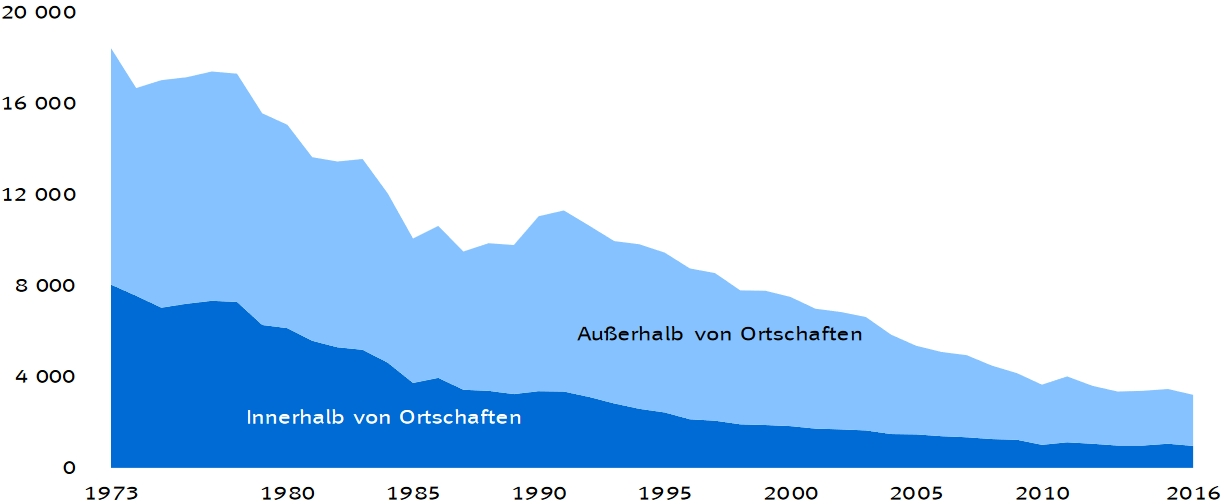
\includegraphics[scale=1.5]{img/Unfalle.jpg}
  \caption{Getötete nach Ortslagen 1973 - 2016\cite{bild1}}
  \label{fig:toteSeit1973}
\end{figure}
Trotz gestiegenem Verkehrsaufkommen sind sowohl die Zahl der Verletzten als auch der getöteten Menschen im Straßenverkehr bis heute stark gesunken. Abb. 1.1 zeigt die Entwicklung der Zahl der Unfallopfer in Deutschland seit dem Jahr 1973. Ein Grund für diesen fallenden Trend sind die eben genannten (und weitere) Fortschritte der Sicherheitssysteme durch die Automobilhersteller. Heute werden die meisten Unfälle durch Fehlverhalten der Fahrer verursacht, wie Abbildung 1.2 verdeutlicht. \\
\begin{figure}[htb]
  \centering  
  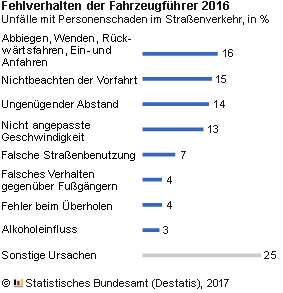
\includegraphics[scale=0.8]{img/Verkehrsunfaelle_Fehlverhalten.jpg}
  \caption{Fehlverhalten der Fahrzeugführer\cite{link}}
  \label{fig:Fehlverhalten}
\end{figure}
Laut Statistischem Bundesamt war im Jahr 2015 menschliches Fehlverhalten des Fahrers zu 88\% aller Unfälle mit Personenschaden die Ursache\cite{bild1}. \\
Dabei liegt in der fortschreitenden Automatisierung die Möglichkeit, Verkehrsunfälle bis auf ein Minimum zu reduzieren. \\
In dieser Bachelor Arbeit wird das Problem behandelt, ein System zu entwickeln, das sich anhand vorgegebener Koordinaten den optimalen Weg zum Ziel sucht und diesen dann möglichst genau abfährt. Die Problematik lässt sich also in zwei Unterprobleme aufteilen, dem Orientieren an einem passenden Pfad, sowie das Abfahren dieses. \\
Autonomes Fahren ist momentan ein Feld in dem viel geforscht wird. Die Automobilhersteller aller Länder liefern sich ein Wettrennen, doch so wie man das aus Science-Fiction Romanen kennt, funktionieren die Autos von heute noch nicht. Diese Arbeit dient der Grundlagenforschung auf diesem Gebiet. \newpage


\section{Problematik}
\label{subsec:problematik}
Um die Bewegung eines dynamischen Systems beschreiben zu können, müssen sich die auf das Fahrzeug wirkenden Kräfte genau angeschaut werden. Aus ihnen lassen sich Kräftegleichgewichte herleiten, mit deren Hilfe man zu den mathematischen Verhaltensbeschreibungen kommt, die möglichst genau die Realität abbilden sollen. 
Dabei lässt sich die Dynamik des Fahrzeugs in zwei Bereiche aufteilen, die Quer- und die Längsdynamik.
Die Freiheitsgrade Nicken und Hieven werden nicht behandelt. Bei der Betrachtung der Querdynamik werden die Bewegungen durch die Reibungskräfte zwischen
Straße und Reifen, sowie Kräfte und Momente der Aerodynamik beeinflusst.
Als Basis für die Regelung- und Steuereinheiten zur Bestimmung der Fahrzeugbewegung gilt
die Sollgrößendefinition, die das Regelziel festlegt. Die Fahrereingaben für das System sind Lenkradwinkel (querdynamisch) und Fahr- beziehungsweise Bremspedalstellung (längsdynamisch). Sie bilden die Basis der Interpretation des Fahrerwunsches, wenn auch nur imaginär, da weder bei der Simulation, noch beim Entwurf Lenker und Pedal tatsächlich enthalten sind. Das gesamte System wird anschließend mittels MATLAB/Simulink simuliert und auf einem RC-Auto mit Raspberry Pi realisiert. 
Diese Arbeit soll einen umfassenden Überblick über bereits veröffentlichte Fahrdynamikkennwerte verschiedener objektiver Fahrmanöver geben. 


\section{Überblick}
\label{subsec:überblick}
\begin{minipage}{0.4\textwidth}
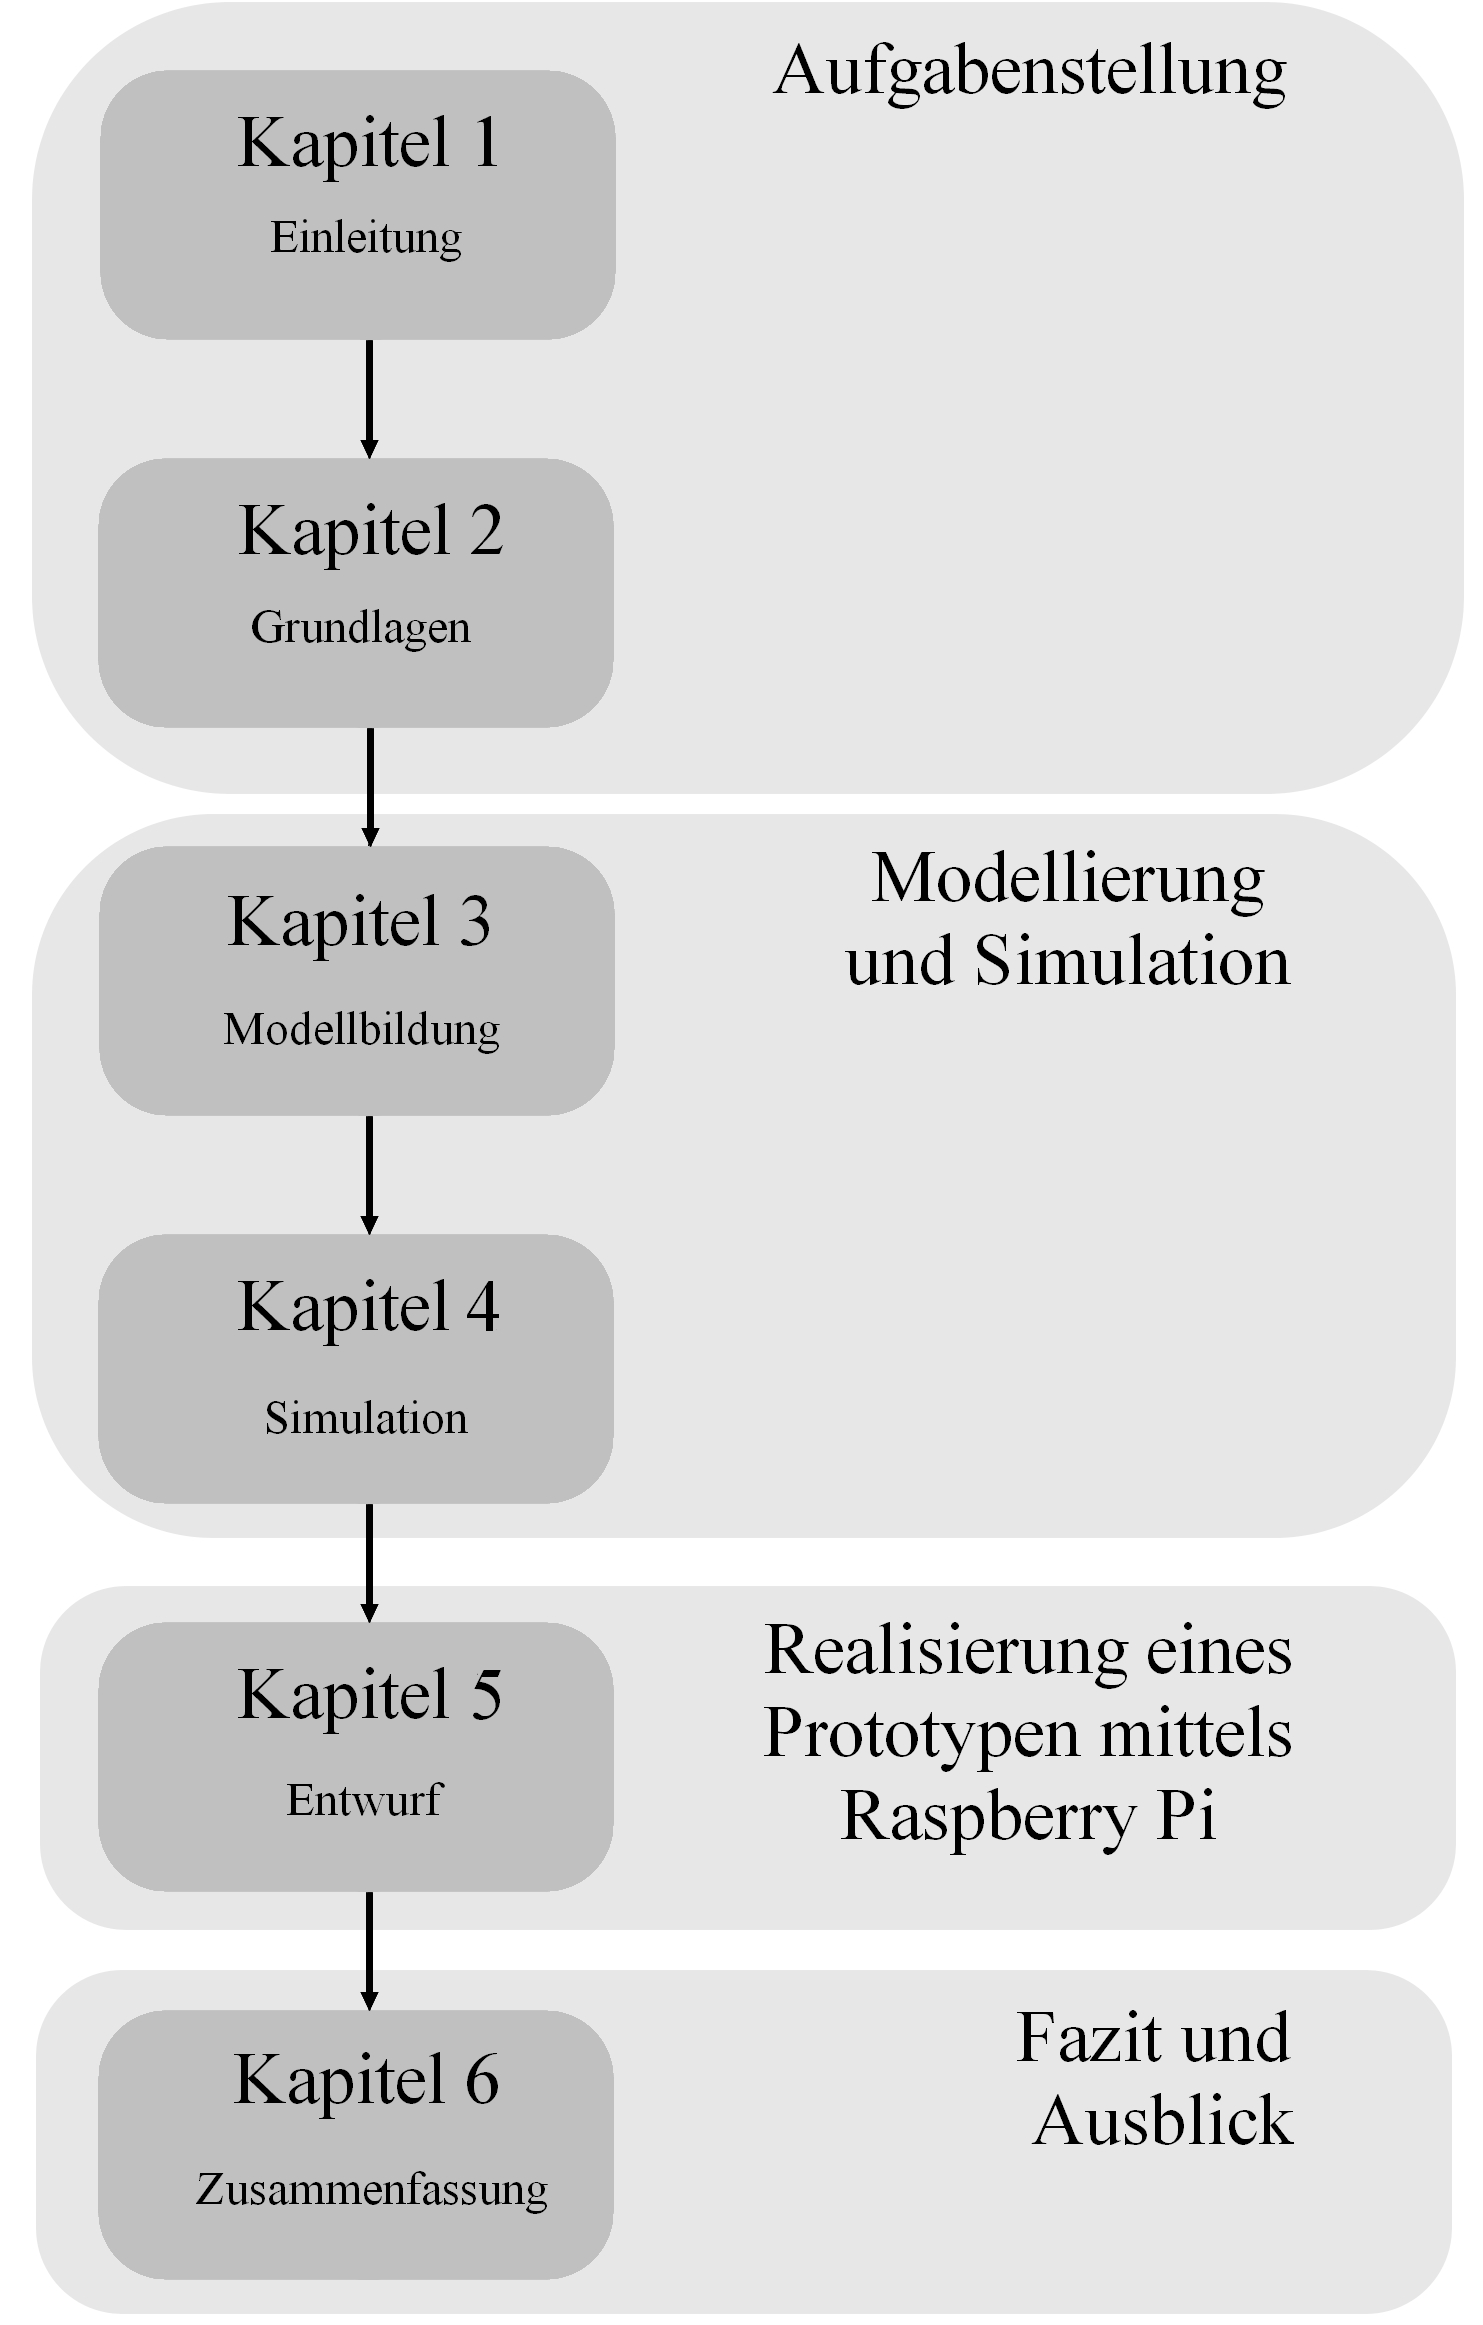
\includegraphics[width=\textwidth]{img/kapitel.jpg}
\end{minipage}
\begin{minipage}{0.6\textwidth}
Die vorliegende Arbeit ist in sechs Kapitel eingeteilt.
Die Kapitel bauen aufeinander auf und sind den einzelnen Teilproblemen der Aufgabenstellung gewidmet. \\
In Kapitel 2 geht es um die mathematischen und physikalischen Grundlagen, die zum Verständnis der folgenden Kapitel notwendig sind.
Kapitel 3 widmet sich der Modellbildung, sprich dem Erstellen mathematischer Formeln, die das Verhalten des Fahrzeugs aus der Aufgabenstellung möglichst realistisch wiedergeben. Es gibt bereits viele bewährte Ansätze und in diesem Fall wird bei dem Fahrzeug von einem Differentialmodell ausgegangen, d.h. einem Fahrzeug mit zwei Rädern und einem Stützrad. Zusätzlich wird hier die Aufgabe der Trajektorienfolgeregelung gelöst, also dem zeitlichen Sollverlauf des Abfahrens verschiedener Wegpunkte auf einem Koordinatensystem. \vspace{.15cm}
\end{minipage}
In Kapitel 4, der Simulation, wird gezeigt wie sich mit Hilfe von MATLAB/Simulink aus dem Modell ein Blockschaltbild erstellen lässt. Das Programm ermöglicht es dann, anhand dieses Blockschaltbilds das Verhalten zu simulieren. Ergebnisse der Simulationen können in dieser Arbeit nur als Bild gezeigt werden, wobei es eigentlich den Fahrvorgang in echtzeit visuell darstellt. In Kapitel 5 wird eine Architektur
entwickelt und die Realisierung eines Prototypen anhand eines Raspberry Pi beschrieben. Fokus hierbei ist die korrekte Ansteuerung der Pins, die wiederum die Aktuatoren des Fahrzeugs steuern sollen.
Im letzten Kapitel wird ein Fazit gezogen und erzielte Ergebnisse kritisch besprochen. Dann schließt diese Bachelorarbeit mit dem Ausblick.


\section{Stand der Technik}
Bislang kennen die meisten das autonome Fahren nur aus Science-Fiction-Büchern oder Filmen, dabei schleichen sich immer mehr autonome Funktionen zum Auto hinzu. So kann der Neuwagen von heute bereits den Abstand zum vorausfahrendem Fahrzeug messen, selbstständig einparken, die Spur halten und noch vieles mehr.
Die Society of Automotive Engineers (SAE) hat das autonome Fahren in sechs international allgemeingültige Stufen eingeteilt, von Level null "Keine Automation" bis zu Level fünf "vollautomatisiert" (vgl. Abbildung 1.3).

Beim Level null ist der Fahrer permanent für sein Fahrzeug verantwortlich, das manuell von ihm gesteuert wird. In Level eins wird der Fahrer von Fahrassistenzsystemen unterstützt, dieses greift aber nicht in Längs- oder Querführung ein. Der Stauassistent ist ein Beispiel für Level zwei, bei dem der Fahrer jedoch noch immer für alles verantwortlich ist (muss bereit sein einzuspringen), obwohl die Fahrzeugführung assistiert ist. Erst ab Level 3 ist es dem Fahrer erlaubt, die Verantwortung zeitweise an das Fahrzeug zu übertragen, muss allerdings aufmerksam bleiben, um für den Fall aller Fälle übernehmen zu können. Bei Level vier sind die ersten Funktionen komplett ohne Fahrer, das jedoch nur in bestimmten Situationen. Z.B. beim Parken oder auf der Autobahn. Das Auto kann in Level fünf in allen Verkehrssituationen auf allen Strecken ohne den Fahrer auskommen. Das Lenkrad ist bei Level fünf obsolet. Aktuell schaffen es die modernsten Autos lediglich auf Stufe 4. \\

Nach einem tödlichen Unfall in Arizona, in dem ein autonom fahrendes Fahrzeug verwickelt war, erlitten die Entwickler von selbst fahrenden Autos einen Rückschlag. Bei dem tragischen Unfall war eine Fußgängerin von einem selbst fahrenden Uber-SUV erfasst und getötet worden. \\
Dieser Vorfall zeigt, dass die Entwicklung am autonomen Fahren noch nicht abgeschlossen ist und unbedingt weitergehen muss. 
\begin{figure}[htb]
  \centering  
  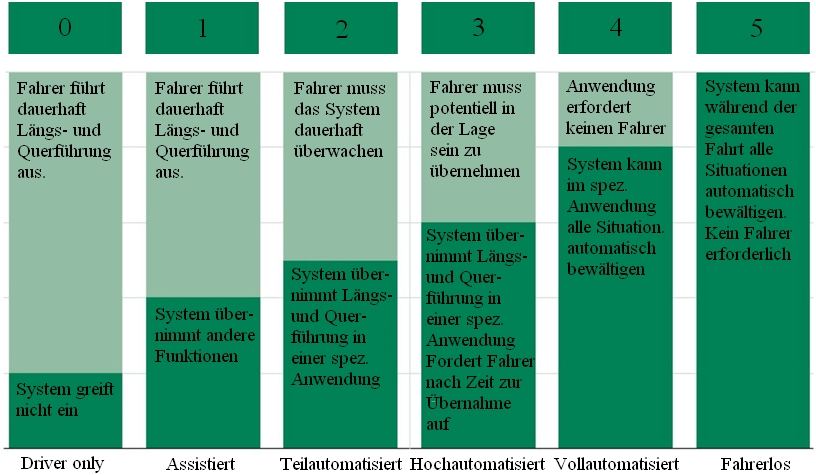
\includegraphics[scale=0.4]{img/automatisierungsgrad.jpeg}
  \caption{die fünf Stufen der Automatisierung}
  \label{fig:die fünf Stufen der Automatisierung}
\end{figure}





\chapter{Grundlagen}
\label{sec:grundlagen}
\section{Zustandsraumdarstellung}
\label{subsec:zustandsraumdarstellung}
Der Zustandsraum ist der Raum, in dem das System durch die Zustandsgrößen aufgespannt wird. Es ermöglicht einen Einblick in das Innere des Systems, indem die im System gespeicherten Energien (Energiemomentaufnahme) erfasst werden und als Matrizen und Vektoren dargestellt werden.
Darstellung im Zeitbereich, d.h. wir gehen von Differentialgleichung des Systems aus. Für die Zustandsraumdarstellung zweiter Ordnung müssen wir die eine Differentialgleichung zweiter Ordnung in zwei Differentialgleichungen erster Ordnung transformieren.
Wir müssen immer eine DG höherer Ordnung erst in mehrere DG erster Ordnung umformen, denn: Bei der Darstellung des Systems spendieren wir pro DG einen Integrator und dieser Integrator kann nur genau einmal integrieren, also nur eine DG erster Ordnung modellieren.
D.h. wir haben nach der Transformation nur DG erster Ordnung.
Dies geschieht indem wir Zustandsvariablen einführen, die einen n-dimensionalen Vektorraum aufspannen, in der dann Zustandstrajektorien gezeichnet werden können. Energiespeicher sind z.B. Masse und Feder. 
\begin{flushleft}
Zustandsgleichung:
$  \vec{\dot{x}} = A\vec{x}+B\vec{u} = $
$
\begin{pmatrix}
a_1 & a_2 & a_3 & a_4 \\
b_1 & b_2 & b_3 & b_4 \\
c_1 & c_2 & c_3 & c_4 \\
d_1 & d_2 & d_3 & d_4
\end{pmatrix}
$ 
\end{flushleft}
\begin{flushleft}
Ausgangsgleichung:
$  \vec{y} = c\vec{x}+d\vec{u} $
\end{flushleft}
Dabei sind: A die Systemmatrix, B die Eingangsmatrix, C die Ausgangsmatrix, D die Durchgangsmatrix. \\
A gibt den Zusammenhang an zwischen Zustandsgrößen $\vec{x}$ und Änderungsgeschwindigkeiten der Zustandsgrößen $\vec{\dot{x}}$. \\
B stellt Zusammenhang her zwischen Eingangsgrößen und Änderungsgeschwindigkeiten der Zustandsgrößen $\vec{\dot{x}}$. \\
C stellt Zusammenhang her zwischen Zustandsgrößen $\vec{x}$ und Ausgangsgrößen $\vec{y}$. \\
D beschreibt, wie die Eingangsgrößen $\vec{u}$ direkt auf die Ausgangsgrößen $\vec{y}$ wirken (Nur bei direkter Verbindung). \\

\section{inverse und direkte Kinematik}
\label{subsec:inverse und direkte Kinematik}
Die direkte Kinematik berechnet in der Robotik aus den Gelenkwinkeln eines Roboters die Pose (Position und Orientierung) und ist damit das Gegenteil der inversen Kinematik, die wiederum aus der Pose die Gelenkwinkel bestimmen kann. Abbildung 2.1 zeigt den Zusammenhang.
\begin{figure}[htb]
  \centering  
  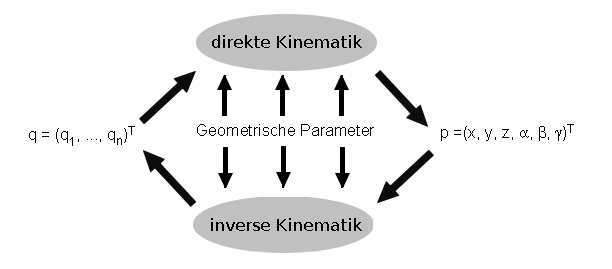
\includegraphics[scale=2.5]{img/Roboterkinematik.png}
  \caption{inverse und direkte Kinematik}
  \label{fig:inverse und direkte Kinematik}
\end{figure}
Bei unserer Arbeit betrachten wir keinen Roboter, sondern ein Fahrzeug, weswegen in unserem Modell aus der Geschwindigkeit des gesamten fahrenden Systems in die Winkel- und die Lineargeschwindigkeit (direkte Kinematik) und zurück (inverse Kinematik) umgerechnet werden kann. Aber dazu in Kapitel 4 genaueres.





\chapter{Modellbildung}
\label{chap:modellbildung}
In unserem Model wird das Nicken und Rollen vernachlässigt, weil wir uns das Fahrverhalten auf einer vertikalen, ebenen Fläche anschauen wollen. 
Die abzufahrende Soll-Strecke soll bestmöglich abgefahren werden. Mittels Regler wird die Differenz der Soll- und der Ist-Werte errechnet. Daraus werden Steuersignale an die Aktuatoren weitergeleitet, die den Kurs oder die Geschwindigkeit korrigieren. Dazu ist es notwendig, die tatsächlichen Werte des Fahrzeuges (wie etwa die Geschwindigkeit oder die Position) zu ermitteln.  

\section{Verwendete Koordinatensysteme}
Zur Beschreibung der Fahrzeugbewegung stehen verschiedene Koordinatensysteme zur Verfügung. Im Folgenden werden die drei Koordinatensysteme vorgestellt: 
\begin{itemize}
\item weltfestes Koordinatensystem $F_w ={x_w,y_w,0}$ 
\item fahrzeugfestes Koordinatensystem auf Höhe des Fahrzeugschwerpunkts $F_f ={P_f,x_f,y_f}$
\item Straßenkoordinatensystem $F_r ={P_r,s_r,d_r}$ 
\end{itemize}
Die einfachste Darstellung der Fahrzeugbewegung geschieht im weltfesten Koordinatensystem $F_w$, in dem die absolute Position des Fahrzeugs abzulesen ist. Ursprung und Ausrichtung sind an einen Ort gebunden und werden durch die Koordinaten $[x_w,yw]$ beschrieben. Das fahrzeugfeste Koordinatensystem $F_f$ hat den Ursprung im Punkt $P_f$, dem Fahrzeugschwerpunkt $s_1$. Es wird durch die Koordinaten $[x_f,y_f]$ beschrieben und ist so orientiert, dass die $x_f$-Achse jederzeit der Fahrzeuglängsachse entspricht und nach vorne gerichtet ist. Die $y_f$-Achse steht entsprechend senkrecht zur Fahrzeuglängsachse und zeigt nach links. Es bewegt sich also mit dem Fahrzeug mit, anders als das weltfeste Koordinatensystem. 
Zum Fahren entlang einer Fahrspur reicht die fahrzeugfeste Position aus, um relativ zur Fahrspur und anderen Verkehrsteilnehmern navigieren zu können. Dazu eignet sich die Darstellung im Straßenkoordinatensystem $F_r$. Mathematisch lässt sich das durch die sog. Frenet-Koordinaten $[s_r,d_r]$ beschreiben. Diese werden durch die Bogenlänge $s_r$ und den Abstand zur Fahrspur $d_r$ beschrieben. Der Tangentenvektort($s_r$)ist dabei immer tangential zum Pfad der Straße ausgerichtet und der Normalenvektor n($s_r$) steht senkrecht dazu und zeigt auf den Referenzpunkt des Fahrzeugs (Fahrzeugschwerpunkt $P_f$).


\section{Bewegungsgleichungen}
Newtons allgemeine Form der Bewegungsgleichung ist
\begin{equation}
  m\cdot a = \sum F  
\end{equation}
Die Massenträgheit ist die Masse multipliziert mit der Beschleunigung und ist auch die Summe aller, von außen wirkenden, Kräfte in dem System.
Bei dem System zum autonomen Fahren handelt es sich dabei um Folgende Kräfte:
\begin{itemize}
\item Zugkraft $F_a = \frac{M}{r} $
\item Straßenwiderstand $F_rr = m\cdot g\cdot C$
\item Luftwiderstand $F_aero = \frac{1}{2}\rho C A V^{2}$
\end{itemize}
Dabei ist $M$ das Drehmoment des Motors, $r$ der Radius eines Rades, $\rho$ die Luftdichte[kg/$m^{3}$], $A$ die Fahrzeugoberfläche orthogonal zur Bewegungsrichtung, $C$ der Koeffizient und $v$ die Geschwindigkeit (Der Luftwiderstand nimmt also quadratisch mit der Geschwindigkeit zu).\\
Setzt man das in die Bewegungsgleichung ein, erhält man
\begin{equation}
  m\cdot a = F_a -  F_rr - F_aero 
\end{equation}
\begin{equation}
  m\cdot a = F_a -  m\cdot g\cdot C - \frac{1}{2}\rho C A V^{2} 
\end{equation}
Teilt man auf beiden Seiten Der Gleichung durch $m$, erhält man die Beschleunigung des Fahrzeugs:
\begin{equation}
  a = \frac{F_a}{m} -  \frac{m\cdot g\cdot C}{m} - \frac{\frac{1}{2}\rho C A V^{2}}{m} 
\end{equation}
\begin{equation}
  a = \frac{F_a}{m} -  g\cdot C - \frac{\frac{1}{2}\rho C A V^{2}}{m} 
\end{equation}
Die Ableitung einer Strecke nach der Zeit ergibt die Geschwindigkeit. Die Ableitung einer Geschwindigkeit nach der Zeit ergibt die Beschleunigung. Sei $x$ die Strecke des Fahrzeugs, dann ist $\dot{x}$ die Geschwindigkeit und $\ddot{x}$ die Beschleunigung.
Damit können wir die Variablen aus der Gleichung ersetzten und erhalten:
\begin{equation}
 \ddot{x} = \frac{F_a}{m} -  g\cdot C - \frac{\frac{1}{2}\rho C A \dot{x}^{2}}{m} 
\end{equation}
So lässt sich leicht erkennen, dass es sich bei dieser Gleichung um eine Differentialgleichung (DGL) zweiter Ordnung handelt. Daraus machen wir jetzt im folgendem Schritt zwei DGL, jeweils erster Ordnung:
\begin{equation}
 x_1=v 
\end{equation}
\begin{equation}
  x_2=\dot{v} 
\end{equation}
Bestimmen von Zustandsvariablen (die Variablen spannen einen Raum im zweidimensionalen Raum, weshalb es so viele Zustandsvariablen gibt, wie es Ordnungen im System gibt):\\
1. Zustandsvariablen miteinander verknüpfen:
\begin{equation}
  \dot{x_1} = x_2 
\end{equation}
2. Einsetzen:
\begin{equation}
  \dot{x_2} = \frac{F_a}{m} -  g\cdot C - \frac{\frac{1}{2}\rho C A {x1}^{2}}{m} 
\end{equation}



\section{Differentialantrieb} 
Wir modellieren das Fahrverhalten anhand eines Fahrzeuges mit zwei Antriebsrädern und einem Stützrad. Gelenkt wird nur über die unterschiedlichen Geschwindigkeiten der einzeln ansteuerbaren Antriebsräder. Wir benutzen zwei Koordinatensysteme, ein Fahrzeugfestes, dessen Ursprung im Fahrzeugmittelpunkt liegt und dessen x-Achse in Richtung des Roboterfrontteils zeigt. die Pose p gibt Auskunft über Position im Weltfesten Koordinatensystem und Winkel zwischen Fahrzeug- und Weltfesten x-Achse.  
\begin{figure}[htb]
  \centering  
  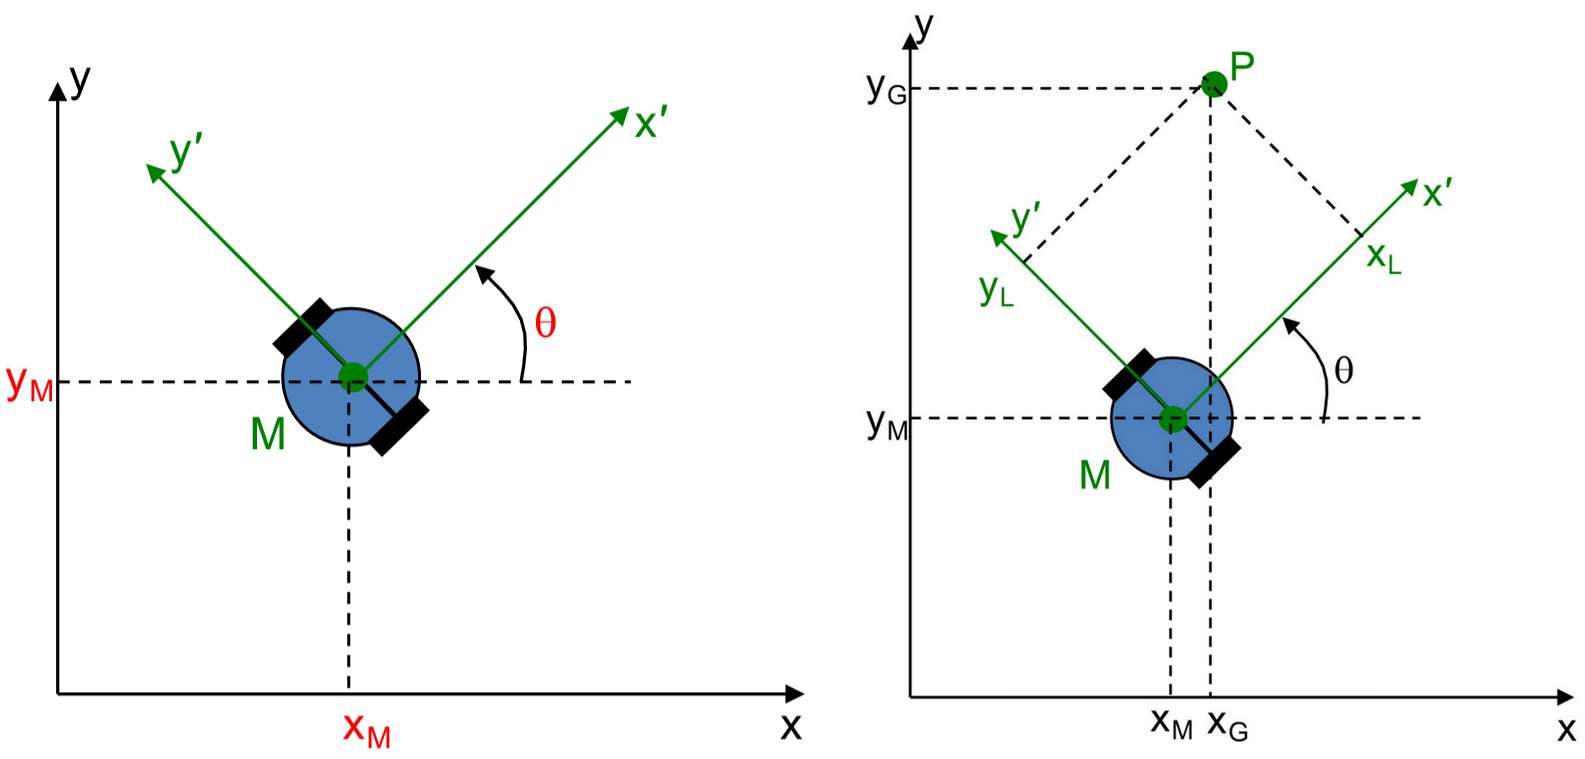
\includegraphics[scale=1]{img/einfachesModell_1.png}
  \caption{Weltfestes- und Fahrzeugfestes Koordinatensystem\cite{robot}}
  \label{fig:Weltfestes- und Fahrzeugfestes Koordinatensystem}
\end{figure}
\begin{equation}
p =
\begin{bmatrix}
x_{weltfest}\\
y_{weltfest}\\
\Theta \\
\end{bmatrix}
\end{equation}
Ein Punkt im Fahrzeugfesten Koordinatensystem F sei: 
\begin{equation}
p_{F} =
\begin{bmatrix}
x_{F}\\
y_{F}\\
\end{bmatrix}
\end{equation}
Der selbe Punkt ist im Weltfesten Koordinatensystem definiert als: 
\begin{equation}
p_{W} =
\begin{bmatrix}
x_{W}\\
y_{W}\\
\end{bmatrix}
\end{equation}
Mit Hilfe der so genannten Rotationsmatrix 
\begin{equation}
R(\Theta) = 
\begin{bmatrix}
cos \Theta & -sin \Theta\\
sin \Theta & cos \Theta\\
\end{bmatrix}
\end{equation}
lässt sich der Punkt aus dem einen in das andere System transformieren: 
\begin{equation}
p_{F} = R(-\Theta)(p_{W}- \begin{bmatrix}
X_{W, fahrzeug} \\
Y_{W, fahrzeug} \\
\end{bmatrix})
\end{equation}
\begin{equation}
p_{W} = R(\Theta)(p_{F}+ \begin{bmatrix}
X_{W, fahrzeug} \\
Y_{W, fahrzeug} \\
\end{bmatrix})
\end{equation}
Die Bewegung unseres Fahrzeugs in der Ebene lässt sich zu jedem Zeitpunkt als Drehung um einen momentanen Drehpunkt auffassen (vergleiche mit Abbildung 3.2), den Momentanpol\cite{robot}. Rotiert das Fahrzeug mit einer Winkelgeschwindigkeit $\omega$ und einem Abstand $r$ um den Momentanpol, dann gilt für die (tangentiale) Geschwindigkeit v in einem Punkt:
\begin{figure}[htb]
  \centering  
  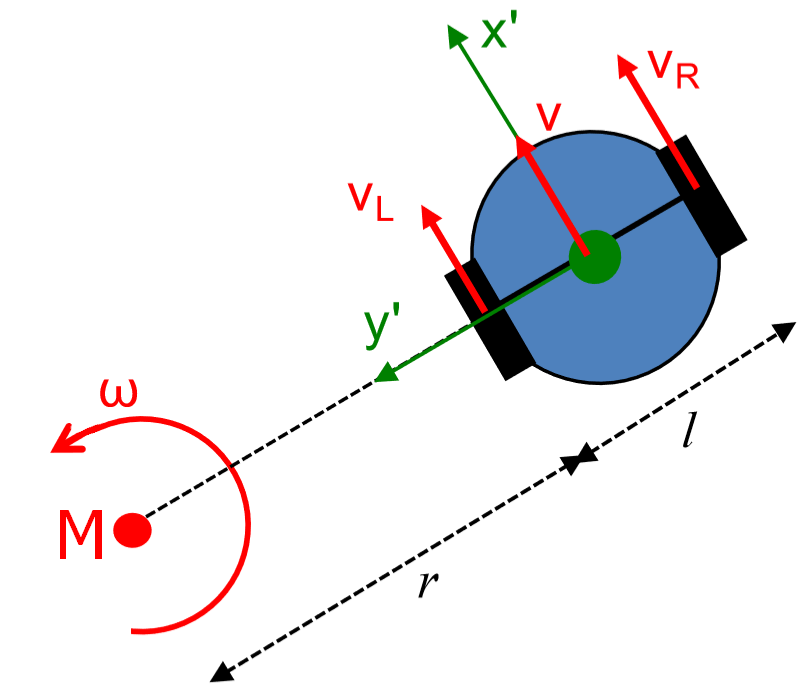
\includegraphics[scale=1]{img/einfachesModell_2.png}
  \caption{Lenkung entspricht Rotation um Momentanpol\cite{robot}}
  \label{fig:Lenkung entspricht Rotation um Momentanpol}
\end{figure}
\begin{equation}
\omega = \frac{v}{r}
\end{equation}
Der Geschwindigkeitsvektor steht dabei senkrecht zu r. Bei Ge­ra­de­aus­fahrt ist die Winkelgeschwindigkeit gleich null und r unendlich groß. \\
Kinematisches Modell: \\
Die Geschwindigkeit des linken Rades $v_{L}$ und die des rechten Rades $v_{R}$ sind voneinander unabhängig. Unser Fahrzeug bewegt sich um den Momentanpol mit Winkelgeschwindigkeit $\omega$ und Geschwindigkeit $v$ in fahrzeugfester x-Richtung.
\begin{equation}
v_{L} = \omega \cdot r
\end{equation}
\begin{equation}
v_{R} = \omega \cdot (r + l)
\end{equation}
Dabei ist $l$ die Breite des Fahrzeugs, sodass der äußerste Punkt des Fahrzeuges den Abstand $r + l$ zum Momentanpol hat. Die Räder haben die gleiche Winkelgeschwindigkeit, aber unterschiedliche Tangentengeschwindigkeiten, weil Ihr Radius sich unterscheidet. Somit hat das Fahrzeug (aufgefasst als Punkt zwischen den Rädern) die Tangentengeschwindigkeit:
\begin{equation}
v = \omega \cdot (r + \frac{l}{2})
\end{equation}
Aus $v_{L}$ und $v_{R}$ und der Achsenlänge $l$ lassen sich $v$ und $\omega$ direkt ermitteln: 
\begin{equation}
v = \frac{v_{R}+v_{L}}{2}
\end{equation}
\begin{equation}
\omega = \frac{v_{R}-v_{L}}{l}
\end{equation}
Ebenso einfach lassen sich $v_{L}$ und $v_{R}$ aus $v$ und $\omega$ bestimmen. \\
In der Realität stellt sich die gewünschte Winkelgeschwindigkeit erst mit einer gewissen Verzögerung ein, aber das lassen wir in unserem Modell unbeachtet. Analoges gilt für die Geschwindigkeit. Konkret kann man also, von den Geschwindigkeiten beider Räder ausgehend, die Geschwindigkeit und Richtung des Fahrzeugs bestimmen. Durch diese Vorgaben berechnet man, wie sich das Fahrzeug verhalten wird. Eventuelle Abweichungen von Soll-Geschwindigkeit und Soll-Richtung können gemessen und an den Regler weitergegeben werden. Dann werden die Differenzen der Soll und Ist Größen von Geschwindigkeit und Lenkwinkel errechnet. Aus den beiden Werten lassen sich dann wiederum $v_{R}$ und $v_{L}$ berechnen, die an die jeweiligen Aktuatoren weitergegeben werden.
\\
Auf einen Punkt zufahren: \\
Um unser Fahrzeug auf einen Punkt $(x_{ziel}$, $y_{ziel})$ zufahren zu lassen, muss eine Geschwindigkeit
\begin{equation}
v = K_{P} \sqrt{(x-x_{ziel})^2 + (y-y_{ziel})^2}
\end{equation}
und eine Zielrichtung 
\begin{equation}
\Theta_{ziel} = atan2(y_{ziel}-y, x_{ziel}-x)
\end{equation}
und eine Winkelgeschwindigkeit 
\begin{equation}
\omega = K_{\omega}\Delta(\theta_{ziel}, \theta)
\end{equation}
passend gewählt werden. Dabei ist $\Delta(\theta_{ziel}, \theta)$ die Winkeldifferenz aus dem Intervall $[-\pi , + \pi]$.\\
Klar ist, dass sich unser Fahrzeug nicht perfekt an die vorgegebenen Trajektorie halten kann. Ziel ist es daher, mittels Regler so nahe wie möglich der Vorgabe zu entsprechen. 
Um einer Linie zu folgen, muss der Abstand zwischen ist und soll auf null reduziert werden.
Je größer die Abweichung, desto größer die Änderung. Mittels PID-Regler wird diese Proportionalität zwischen Abstand und Winkelgeschwindigkeit erzeugt: 
\begin{equation}
\omega(t) = \underbrace{-K_{P}e(t)}_{\substack{P}} - \underbrace{-K_{I}\int {e(t)dt}}_{\substack{I}} - \underbrace{-K_{D}\frac{de(t)}{dt}}_{\substack{D}}
\end{equation}
Einstellen der Parameter $K_{P}, K_{I}, K_{D}$ mittels Faustregel (z.B. Ziegler/Nichols).














\section{Trajektorienfolgeregelung}
\label{sec:trajektorienfolgeregelung}
Zum Fahren braucht ein Fahrzeug eine Strecke, auf der es von Punkt A nach Punkt B gelangt. In unserem Modell soll sich das Fahrzeug selbst den Weg suchen, um das vorgegebene Ziel zu erreichen. In diesem Kapitel wird die autonome Berechnung einer \textit{Trajektorie} behandelt. 
Eine Trajektorie ist der geplante Sollverlauf der Fahrzeugszustandsgrößen \cite{trajDef}, beziehungsweise eine Kurve in der Ebene, parameterisiert über die Zeit. Die einzelnen Punkte der Kurve sind die Positionen zu bestimmten Zeitpunkten. Ohne die dazugehörigen Zeitinformationen, ist die Trajektorie nur ein Pfad. Dabei ist die Orientierung die Tangente des jeweiligen Punktes.
Ergebnis der Trajektorienplanung ist der zu fahrende Verlauf. Als Vorgaben erhält das Fahrzeug dafür die Koordinaten des Ziels und (gegebenenfalls) Hindernisse. 
Die aktuelle Trajektorie gibt die aktuelle Geschwindigkeit in x- und y-Richtung an.
Um aus diesen Informationen einen Pfad aussuchen zu können, der zum Ziel führt, muss es ein Bewertungsschema geben. Es gibt unendlich viele Wege, aus denen das Fahrzeug wählen kann, aber nur einen kürzesten. Das Kriterium für einen guten Pfad ist also äquivalent zu seiner Länge. Ohne Hindernisse ist das einfach eine Gerade vom Ausgangspunkt zum Ziel, und das Fahrzeug kann ohne Regelung die Aufgabe erledigen.
Mithilfe von Matlab lässt sich eine Simulation entwickeln, die den Pfad zwischen Start und Ziel auf einem zweidimensionalen Koordinatensystem zeigt \cite{ml}. 
\lstset{language=Matlab}          
\begin{lstlisting}[frame=single]
%% EXAMPLE: Differential Drive continuous simulation
R = 0.1;                % Wheel radius [m]
L = 0.5;                % Wheelbase [m]
dd = DifferentialDrive(R,L);

%% Run a continuous simulation using ODE45
initPose = [0 0 pi/4];  % Initial pose (x y theta)
tspan = [0 10];
[t,pose] = ode45(@(t,y)diffDriveDynamics(t,y,dd),tspan,initPose);
pose = pose';

%% Display results
close all
figure
hold on
plot(pose(1,1),pose(2,1),'ro', ...
     pose(1,end),pose(2,end),'go', ...
     pose(1,:),pose(2,:),'b-');
axis equal
title('Vehicle Trajectory');
xlabel('X [m]')
ylabel('Y [m]')
legend('Start','End','Trajectory')


%% Continuous dynamics
function dy = diffDriveDynamics(t,y,vehicle)
    
    % Set desired velocities and solve inverse kinematics
    vDes = 0.2;
    if t < 5
       wDes = -0.5; 
    else
       wDes = 0.5;
    end
    [wL,wR] = vehicle.inverseKinematics(vDes,wDes);
    
    % Calculate forward kinematics and convert the speeds to global
    [v,w] = vehicle.forwardKinematics(wL,wR);
    velB = [v;0;w];            % Body velocities [vx;vy;w]
    dy = bodyToWorld(velB,y);  % Convert from body to world
end
\end{lstlisting}
Durch Ausführung dieses Codebeispiels in Matlab wird das in Abbildung 3.3 gezeigte Bild erzeugt. 
\begin{figure}[htb] 
  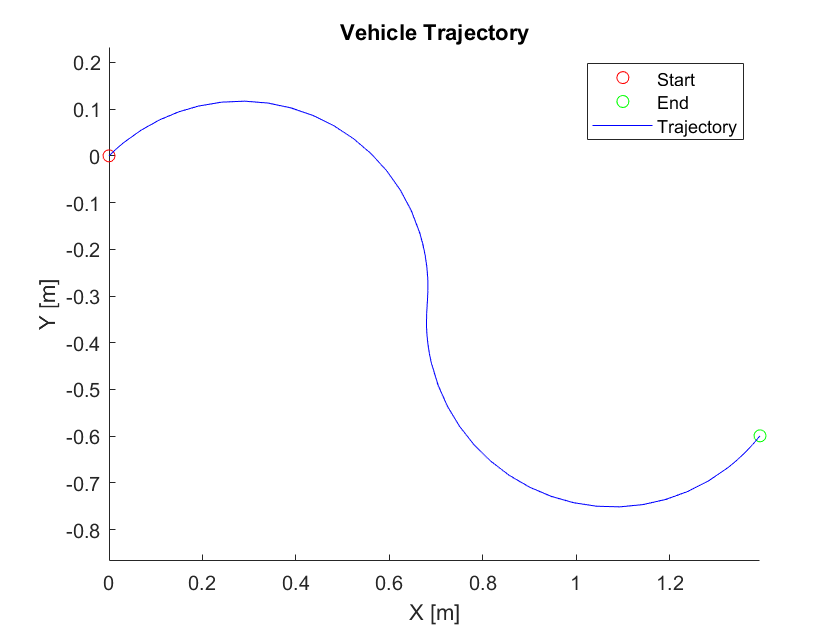
\includegraphics[scale=0.8]{img/einacherPfad.png}
  \caption{MATLAB Beispiel}
  \label{fig:MATLAB Beispiel}
\end{figure}
Bei diesem Modell wird der 'pure pursuit path tracking' (pure Verfolgung) Algorithmus verwendet, um nacheinander die auf einem Weltfestem Koordinatensystem vorhandenen Wegpunkte abzufahren. Bei der puren Verfolgung handelt es sich um eine bewährte Methode, die sich bildhaft mittels Karotte und Esel veranschaulichen lässt. Eine Karotte ist in einem festen Abstand zum Esel an dem Esel befestigt. Der Esel sieht die Karotte vor sich und während er ihr sich vermeintlich nähert, bewegt sie sich mit der gleichen Geschwindigkeit, von ihm weg. Bei der puren Verfolgung bewegt sich ein Zielpunkt über die gewünschte Strecke, die in diesem Fall einfach eine Gerade zwischen Fahrzeug und Ziel ist. Der PID-Regler sorgt dafür, dass das Fahrzeug einen konstanten Abstand zum dynamischen Zielpunkt beibehält. Das Fahrzeug jagt also einem auf dem Pfad entlang verlaufenden Punkt hinterher. Ein weiterer Regler ist für die Ausrichtung des Fahrzeugs in dynamische Zielrichtung verantwortlich. Das bedeutet, dass das Fahrzeug nur genau dann schneller als das dynamische Ziel ist, wenn die Ausrichtung nicht zum Ziel ist. \\
Bei passend gewählter Geschwindigkeit, Winkelgeschwindigkeit und Abstand zum dynamischen Zielpunkt, nähert sich der Ausrichtungswinkel in immer kleiner werdenden Anpassungen, dem Pfad an, ohne ihn zu überschreiten und wieder zurück lenken zu müssen. Dafür müssen die Geschwindigkeiten antiproportional zum Abstand zum dynamischen Ziel sein. \\
Kurz gefasst kann man die Pure Verfolgung in folgenden Schritten skizzieren, die ständig der Reihe nach abgearbeitet werden:
\begin{itemize}
\item aktuelle Pose des Fahrzeugs bestimmen
\item den dynamischen Zielpunkt finden
\item die Zielpunktkoordinaten in Fahrzeugkorrdianten transformieren
\item das Fahrzeug darauf zufahren lassen [Link zur Textstelle in der Modellierung in der das genauer erleutert wird]
\end{itemize} 
\begin{figure}[htb]
  \centering  
  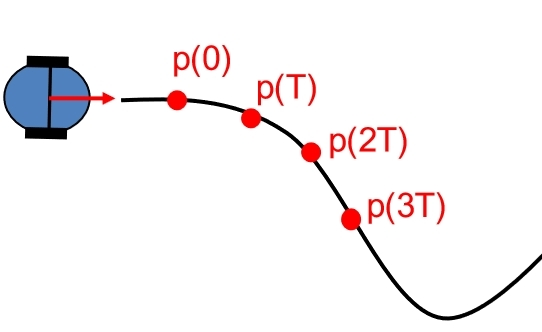
\includegraphics[scale=1.4]{img/purePursuit.jpg}
  \caption{Pure Pursuit Veranschaulichung\cite{robot}}
  \label{fig:starwars}
\end{figure}
Dieses Kapitel war geprägt von mathematischer Modellierung und Herleitung gesuchter Gleichungen aus der Physik. Als Resultat konnte ein Fahrzeugmodell entwickelt werden, das sich anhand von Eingabeparametern, auf Längs- und Querdynamik simulieren lässt, wie im nächsten Kapitel vorgemacht.\\

\chapter{Simulation}
\label{sec:simulation}
Im diesem Kapitel wird die Simulation anhand von MATLAB/Simulink (Version R2018a) dargestellt. Dabei werden die Fahrparameter dynamisch berechnet. Um dies zu erreichen wurde das Modell für den Differentialantrieb aufgebaut, um Vorhersagen über das Fahrverhalten treffen zu können. 
Die modellbasierte Simulation erlaubt es Fahrdynamikregelsysteme zu entwickeln, ohne teure Tests unternehmen zu müssen. Abbildung 4.1 verdeutlicht den Unterschied der in diesem Kapitel vorgestellten Regelungsarten, die beide in unserem Modell gebraucht werden.

\begin{figure}[htb]
  \centering  
  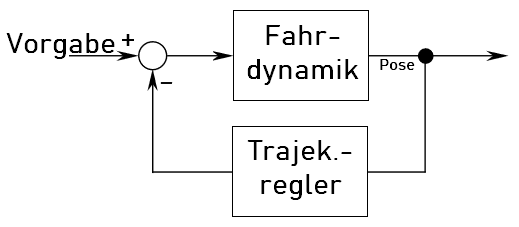
\includegraphics[scale=2]{img/vier.png}
  \caption{Zusammenwirken des Dynamischen Reglers (Kapitel 4.1) und des Trajektorien Reglers (Kapitel 4.2)}
  \label{fig:Zusammenwirken des Dynamischen Reglers (Kapitel 4.1) und des Trajektorien Reglers (Kapitel 4.2)}
\end{figure} 


\section{Dynamische Regelung}
Abbildung 4.2 zeigt das einfachere Fahrzeugmodell im Blockschaltbild samt Regler. In dem oberen Kasten erfolgt die Berechnung der Geschwindigkeit und der Winkelgeschwindigkeit aus den beiden Radgeschwindigkeiten. Als Ausgabe erhält man die aktuellen Werte, die in dem Regler mit den Soll-Werten aus der Trajektorie verglichen werden. Aus Gründen der Übersichtlichkeit übernimmt der Regler zusätzlich die Aufgabe des Umrechnens der Regelgrößen. Als Ergebnis bekommt man also die Stellgrößen für die Geschwindigkeit der beiden Räder heraus, die an die Aktuatoren weitergegeben werden. Im nun folgenden Modell nehmen wir jedoch nicht die beiden Radgeschwindigkeiten als input, sondern die lineare- und Winkelgeschwindigkeit. \\
\begin{figure}[htb]
  \centering  
  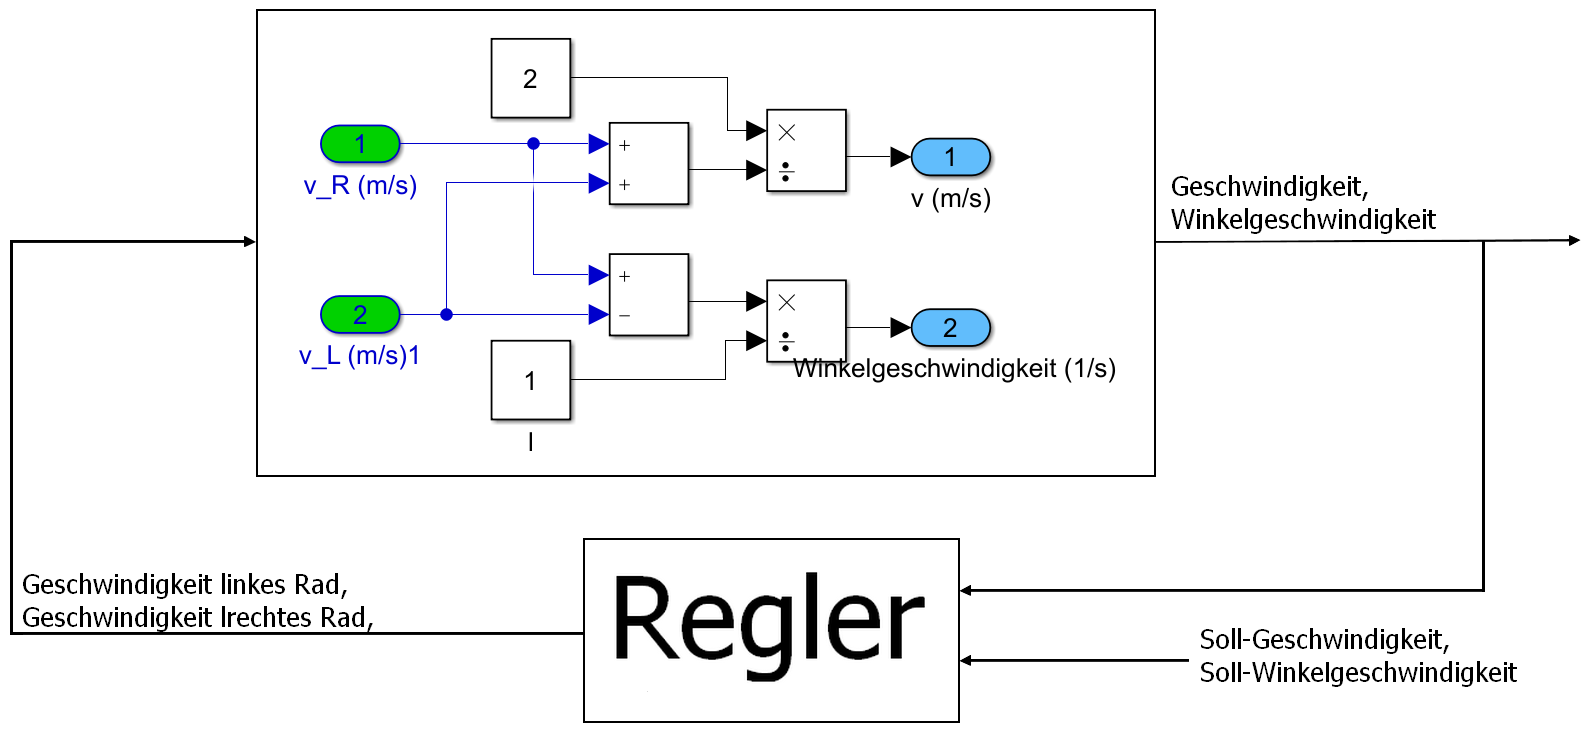
\includegraphics[scale=1]{img/Blockschaltbild1.png}
  \caption{Logischer Aufbau unseres Modells}
  \label{fig:starwars}
\end{figure}
Mithilfe von Simulink lässt sich eine Simulation erstellen, anhand derer man sich vergewissern kann, dass das in Kapilel 3 erstellte mathematische Modell tatsächlich so funktioniert, wie erwartet. Abbildung 4.3 zeigt das zur Simulation dazugehörige Blockschaltbild. Als Eingabe wird die (Tangenten-)Geschwindigkeit und die Winkelgeschwindigkeit bestimmt. Durch die inverse Kinematik werden anhand dieser Eingangsgrößen die Geschwindigkeiten beider Räder berechnet, die selbst schon ein Ausgangssignal bilden (Pfeil nach unten). Folgt man dem Pfeil nach oben, so wird aus den beiden Radgeschwindigkeiten wieder in Geschwindigkeit und Winkelgeschwindigkeit transformiert, mittels direkter Kinematik. Bei dem mittleren Pfeil wird aus den Radgeschwindigkeiten die Pose des Fahrzeugs ermittelt. \\
An den beiden Reglern lassen sich die Eingangsgrößen Geschwindigkeit und Winkelgeschwindigkeit verstellen, was sich unmittelbar in der Simulation auswirkt, sodass man sofort eine visuelle Rückmeldung für die veränderten Größen bekommt. Ändert man die Werte nicht, so bleibt die Geschwindigkeit und die Tangentengeschwindigkeit konstant, was eine Kreisbewegung des Fahrzeugs zur Folge hat (für $\omega \not= 0$). Da an dieser Stelle noch keine vorgegebene Trajektorie abgefahren werden soll, gibt es auch keinen Regler.
\begin{figure}[htb]
  \centering  
  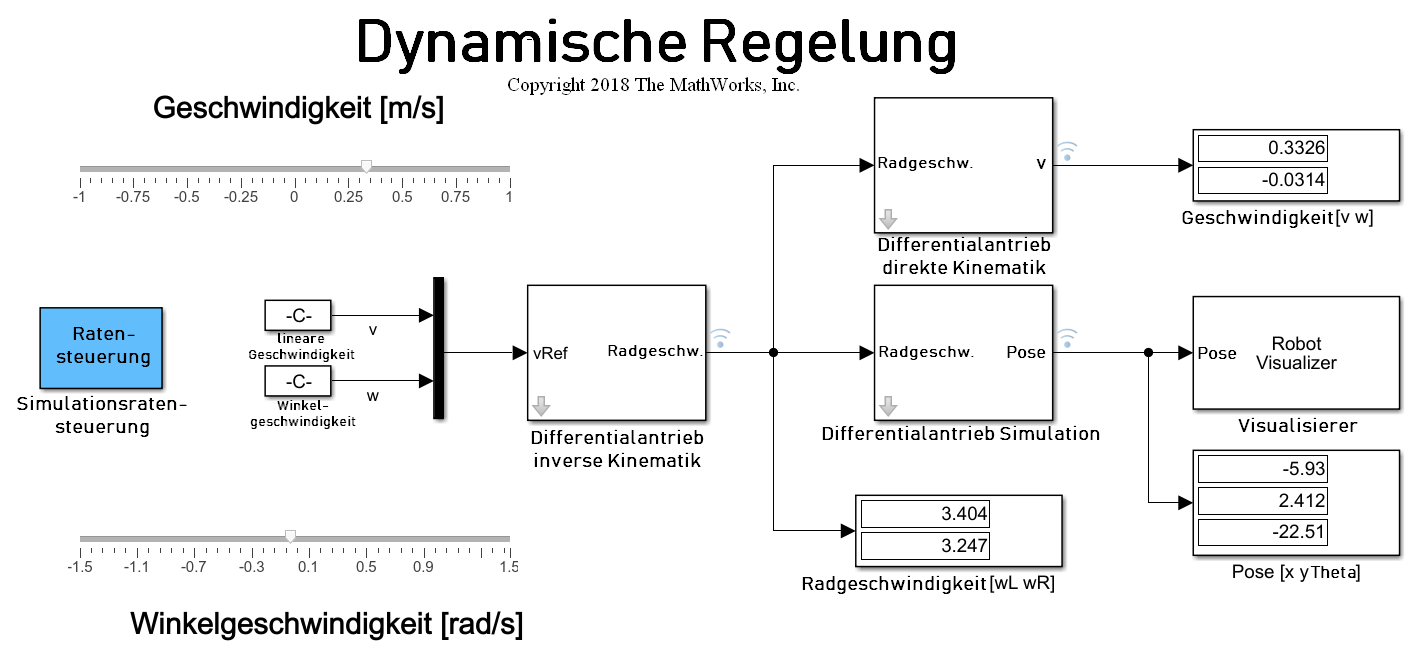
\includegraphics[scale=1.4]{img/simulation1.png}
  \caption{Simulation - Blockschaltbild einfaches Modell}
  \label{fig:starwars}
\end{figure}
Als Beispiel für das Ergebnis dieser Simulation, ist in Abbildung 4.5 eine selbsterklärende Momentaufnahme zu sehen. Die Abstände der einzelnen Punkte zueinander geben Hinweise auf die aktuelle Geschwindigkeit, und die Kreisbahn ist abhängig von der gewählten Winkelgeschwindigkeit. \\
\begin{figure}[H]
  \centering  
  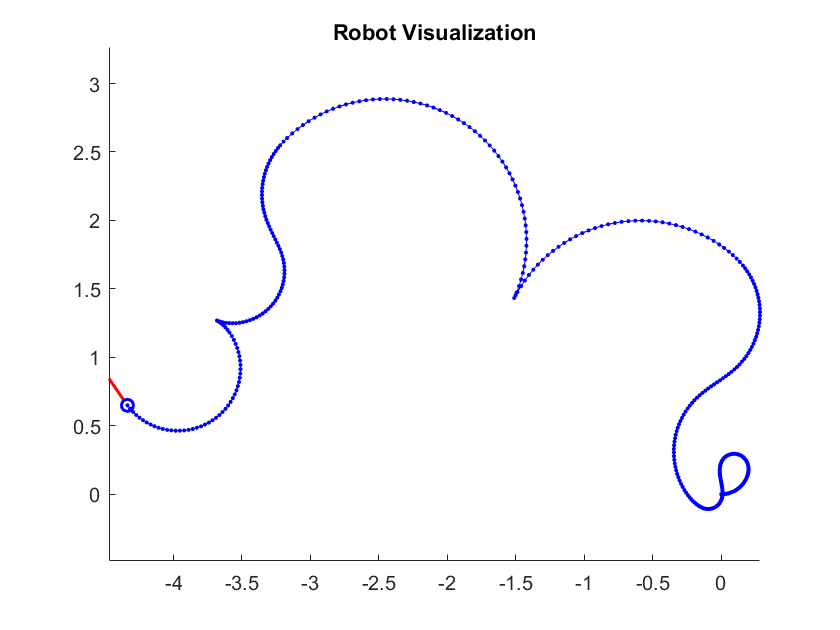
\includegraphics[scale=0.7]{img/simulationsergebnis2.png}
  \caption{Simulation - Ergebnis der Simulation der Kinematik}
  \label{fig:starwars}
\end{figure}

\section{Trajektorien Regelung}
Ein weiteres Blockschaltbild (Abbildung 4.5) simuliert das Verhalten des gleichen Fahrzeugs beim Abfahren verschiedener vorgegebener Punkte mittels Regler, sprich der Trajektorienregelung. Das Ergebnis wird in Abbildung 4.6 veranschaulicht. Die leichten Abweichungen liegen an der Regelung und an dem gewählten Maximalabstand, ab dem ein Zielpunkt als erreicht gilt.
\begin{figure}[htb]
  \centering  
  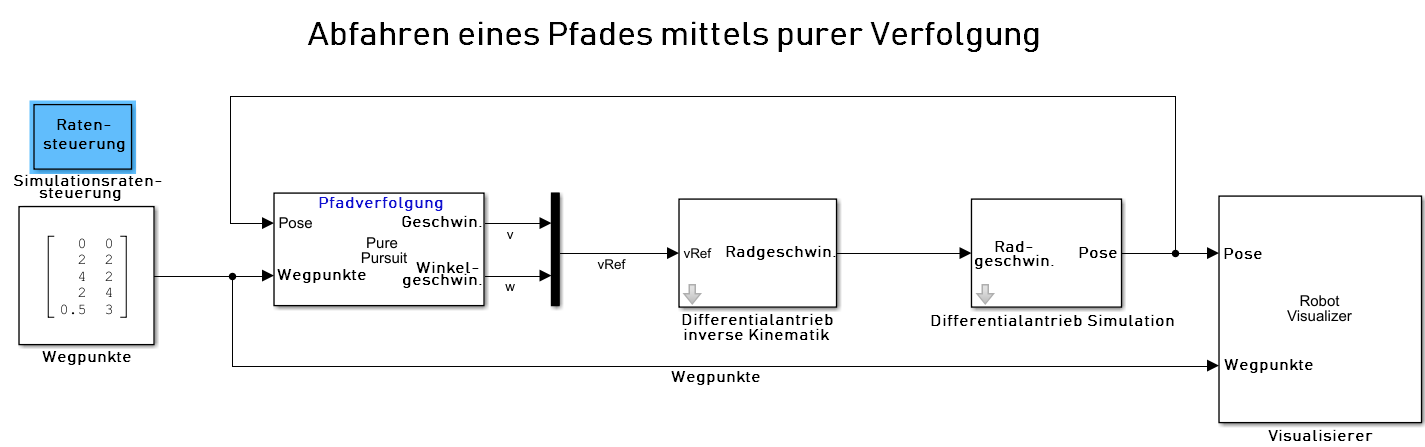
\includegraphics[scale=1.4]{img/einfachesmodellpunkteanfahrensimulation.png}
  \caption{Simulation - Vorgegebene Koordinaten abfahren}
  \label{fig:starwars}
\end{figure}

In dieser Simulation soll ein möglichst kurzer Pfad zwischen aktueller Position des Fahrzeugs und dem Ziel bestimmt werden. Möglichst kurz ist hier gleichzusetzen mit möglichst wenig Lenkung, was zu einer 'geraderen' Strecke führt. \\
Anders als bei vorherigen Simulation, spielen hier auch die Trajektorienplanung und die dynamische Regelung entscheidende Rollen. \\
Da man nur ein paar abzufahrende Punkte hat und nicht etwa eine alles verbindende Streckenvorgabe, muss der Pfad bestimmt werden bevor sich das Fahrzeug in Bewegung setzt.  

\begin{figure}[H]
  \centering  
  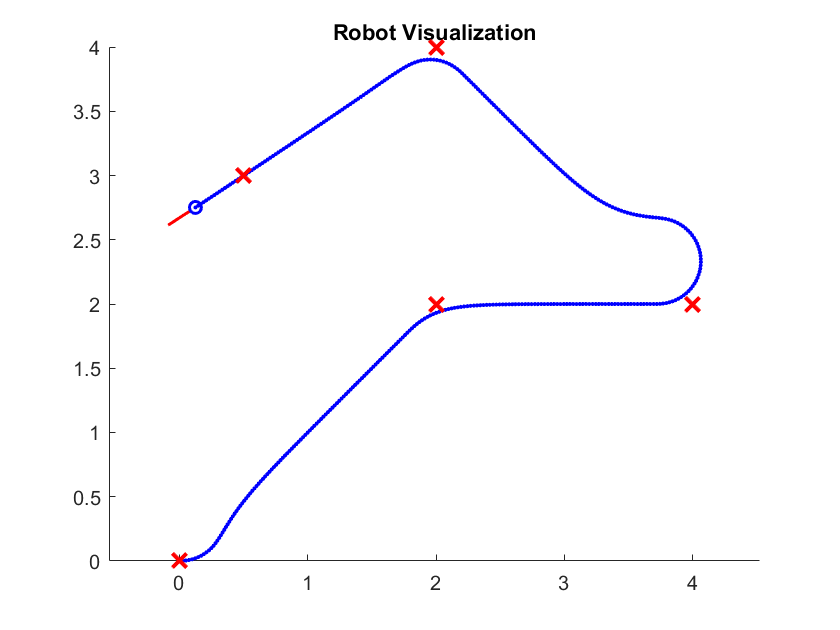
\includegraphics[scale=0.7]{img/simulationsergebnis1.png}
  \caption{Simulation - Ergebnis Punkte abfahren}
  \label{fig:starwars}
\end{figure}

Im folgendem Kapitel wird mittels Raspberry Pi ein Prototyp realisiert. Dies geschieht über die Software-Hardware-Schnittstelle, die das digitale Ansteuern von Analogen Aktuatoren ermöglicht.






\chapter{Entwurf}
\label{sec:entwurf}


\section{Raspberry Pi}
Zur Überführung des Systems in die Realität benutze ich Raspberry Pi Version B als Schnittstelle zwischen Computermodell und der Umsetzung auf Hardware samt Aktuatoren (Motoren, Regler usw.). Dieser gibt die Steuersignale direkt an die Aktuatoren weiter, die letztlich die Geschwindigkeit und Lenkung bestimmen. 
Raspberry Pi ist ein kostengünstiger Einplatinen-Computer, der in etwa die Größe einer Kreditkarte hat und auf dem Linux-Betriebssysteme laufen. Raspberry Pi basiert auf ARM® Cortex® A-Prozessoren und hat verschiedene Ausgänge für Verbindungen mit Peripheriegeräten wie Stereo-Audio, digitales Video, USB und Ethernet.


\section{Realisierung auf dem RaspberryPi}
\label{sec:Umsetzung}
Bei Matlab/Simulink können Modelle mit Hilfe der richtigen Support Packages direkt auf der Hardware (den Raspberry Pi 2 Version B) ausgeführt werden. Dabei unterscheiden sich Matlab und Simulink wie folgt: \\
Mittels Ethernetkabel werden bei der Ausführung von Modellen in Matlab Daten von der Hardware eingelesen oder Informationen zur Hardware gesendet.
Anders als bei Matlab wird bei Simulink der Algorithmus direkt auf der Hardware ausgeführt.
Dazu generiert das Simulink Support Package beim Ausführen des Modells Code, der anschließend auf dem Raspberry Pi ausgeführt wird.
Mit dem Simulink Support Package für Raspberry Pi lassen sich Algorithmen entwickeln, die eigenständig auf dem Raspberry Pi ausgeführt werden können. Das Support Package erweitert Simulink um Blöcke, mit denen sich die digitale Pins des Raspberry Pi steuern lassen, sowie Daten eingelesen und geschrieben werden können. Hat man erst ein funktionierendes Simulink-Modell erstellt, lässt sich der dazugehörige Algorithmus auf den Raspberry Pi herunterladen und dort eigenständig ausführen. \\
Mittels Support Package kann über eine Remote Verbindung mit dem Raspberry Pi kommuniziert werden. Dieser steuert Peripheriegeräte und kann Daten von Sensoren einlesen. MATLAB arbeitet auf dem Raspberry Pi nicht als Standalone, denn der MATLAB-Code wird nicht lokal auf der Hardware ausgeführt. \\
Die General-Purpose-Input-Outputs (GPIO) können nur boolsche Werte annehmen. Sie dienen ausschließlich der logischen Signalweitergabe und nicht als Strom oder Spannungsquelle. \\
Servomotoren können mit einem einzigen GPIO gesteuert werden. Die Rotation und der damit resultierende Lenkwinkel entstehen durch die Dauer des Impulses am Pin. Der Winkel hängt dabei vom spezifischen Servo ab. \\
\\

Die GPIO bilden die Schnittstelle zwischen dem Raspberry Pi und digitalen Schaltungen. Nachdem man über die Konsole in MATLAB Verbindung zu der Hardware aufgebaut hat, lässt sich via PuTTY eine Konsole öffnen, in der man interaktive Befehle auf dem Raspberry Pi ausführen lassen kann:
\lstset{language=bash}          
\begin{lstlisting}[frame=single]
rpi = raspi();
openShell(rpi)
\end{lstlisting}
Nach dem Einloggen auf der Hardware, lassen sich die einzelnen GPIO austeuern. Diese befinden sich als Dateien im Verzeichnis /sys/class/gpio. Um einen Pin ansteuern zu können, muss man ihn vorher 'exportieren'. Im folgendem Beispiel wird das an Pin 17 demonstriert:
\lstset{language=bash}          
\begin{lstlisting}[frame=single]
echo "17" > /sys/class/gpio/export
\end{lstlisting}
Dadurch wird ein neuer Ordner innerhalb von /sys/class/gpio/gpio17/ erstellt, mit dem nun gearbeitet werden kann. Das geschieht, indem man den Pin als Input oder als Output definiert, also ob man Signale lesen oder schreiben möchte: 
\lstset{language=bash}          
\begin{lstlisting}[frame=single]
echo "out" > /sys/class/gpio/gpio17/direction
\end{lstlisting}
Der GPIO ist binär. Er kann entweder eine Spannung von 3,3 Volt haben, oder keine. Er kann lediglich diese beiden Zustände annehmen und lässt sich nun ansteuern:
\lstset{language=bash}          
\begin{lstlisting}[frame=single]
echo "1" > /sys/class/gpio/gpio17/value
\end{lstlisting} 

Alternativ lassen sich die GPIO auch über WiringPi steuern. WiringPi ist ein Framework, das die Einbindung in Programmiersprachen wie Python oder C ermöglicht.  
Darüber hinaus kann es mit den mitgelieferten Bibliotheken in C, C++, Python, Java und php eingebunden werden. Es benutzt eine andere GPIO-Belegung, aber durch die Option -g wird die normale Raspberry Pi Belegung genutzt. Es lassen sich die gleichen Befehle ausführen, aber mit anderem Syntax:
\lstset{language=bash}          
\begin{lstlisting}[frame=single]
gpio export 17 out 
gpio -g write 17 1 
\end{lstlisting}
Der eigentliche Vorteil liegt aber darin, dass eine Bibliothek von Befehlssätzen, die mit WiringPi installiert werden, in C-Code integriert werden kann, wodurch sich mit der Programmiersprache direkt die Pins ansteuern lassen. Weil auch unser Modell aus Simulink in C-Code kompiliert wird, besteht hier die Möglichkeit, diese beiden losen Fäden zu verbinden. \\
Bei jedem Simulink Modell, das erfolgreich auf dem Raspberry Pi läuft, wird eine ELF (Executable and Linking Format) erstellt. \\ \\

Testweise wurde ein MOSFET an den GPIO 17 angeschlossen. Dieser dient als Schalter: Liegt eine Spannung am richtigen der drei Eingänge des MOSFETs an, so schließt sich der Schalter zwischen den zwei anderen Eingängen und Strom kann fließen. An dem MOSFET waren noch eine LED sowie eine Stromquelle angeschlossen. Solange an dem Pin eine logische 0 anlag, passierte nichts, aber durch die Veränderung des Wertes, schloss der MOSFET den Stromkries und das LED leuchtete (vgl. Abbildung 5.1). \\
\begin{figure}[htb]
  \centering  
  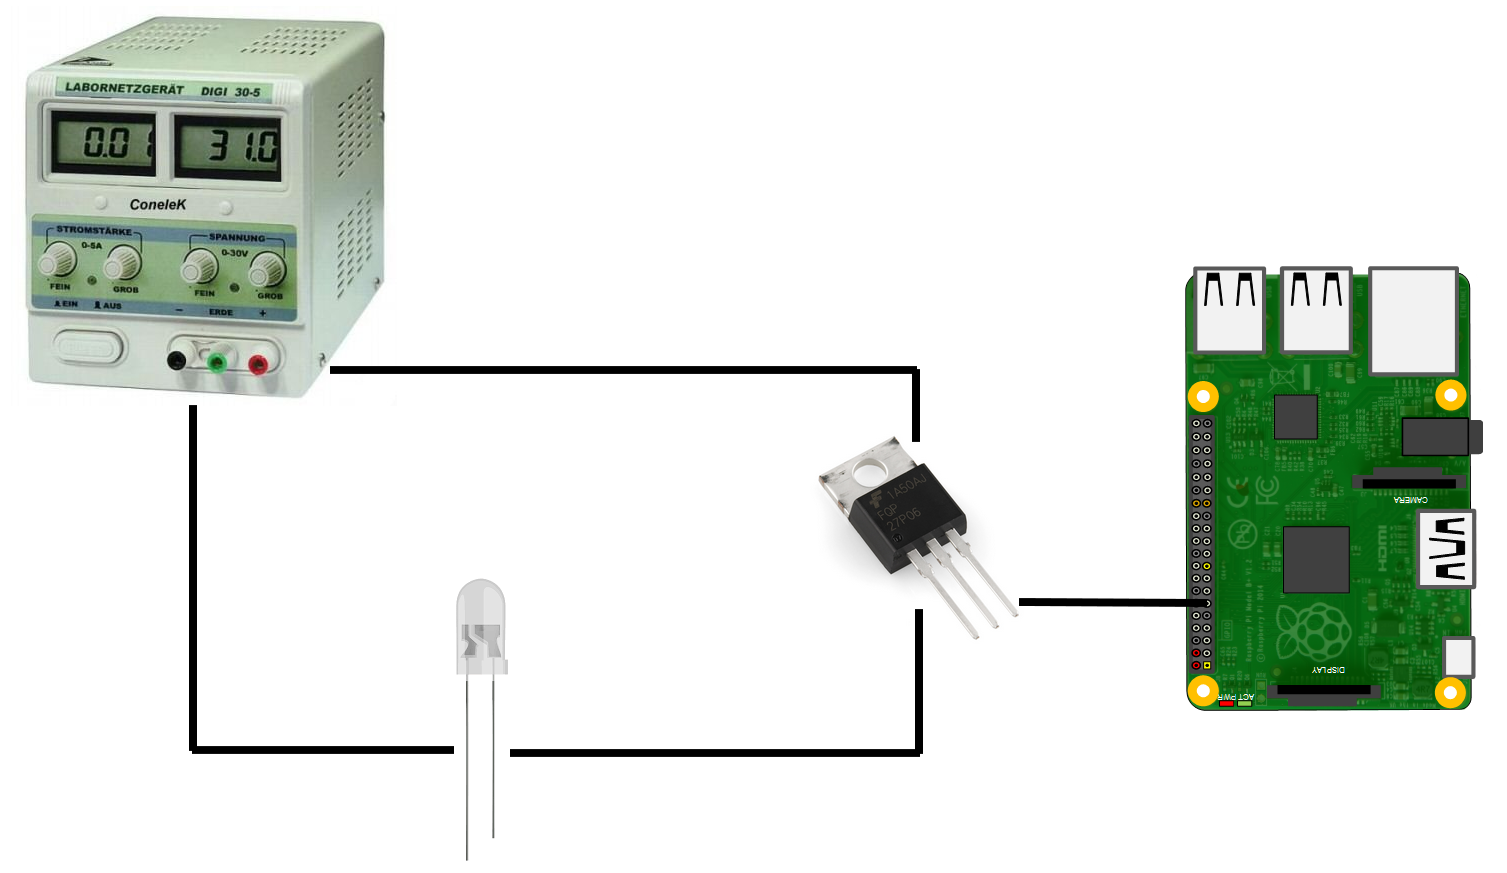
\includegraphics[scale=1]{img/versuchsaufbau.png}
  \caption{Versuchsaufbau der Ansteuerung des GPIO 17}
  \label{fig:starwars}
\end{figure}


Die nächste Überlegung war, wie man überhaupt anhand von Signalen Motoren steuern kann. Zur Lenkung empfiehlt sich ein Servo-Motor, der im Gegensatz zu Schrittmotoren bereits mit einem Pin auskommt und über die Länge des Impulses den Lenkwinkel bestimmen kann, allerdings wird in unserem gewähltem Fahrzeugmodell die Lenkung über die unterschiedlichen Geschwindigkeiten beider Räder bestimmt, also braucht man einen Schrittmotor. Am besten werden Motoren über PWM (Pulsweitenmodulation) geregelt, womit wiederholte Signale in regelmäßigen Abständen übertragen werden. Das kann man sich so vorstellen: Das Signal, also die Spannung am GPIO, wird getaktet. In gleichmäßigen Abständen wechselt es zwischen 1 und 0, zwischen an und aus, also ob 3,3 Volt anliegen oder nicht. Dadurch lässt sich die durchschnittliche Spannung regulieren. Ist der Impuls/Pulsweite kurz, gibt es einen Längeren Zeitraum, in dem keine Spannung anliegt, und der Motor sollte langsamer werden. Um das veranschaulich zu verifizieren wurde ein weiteres Simulink Modell gebaut (siehe Abbildung 5.2). \\
\begin{figure}[htb]
  \centering  
  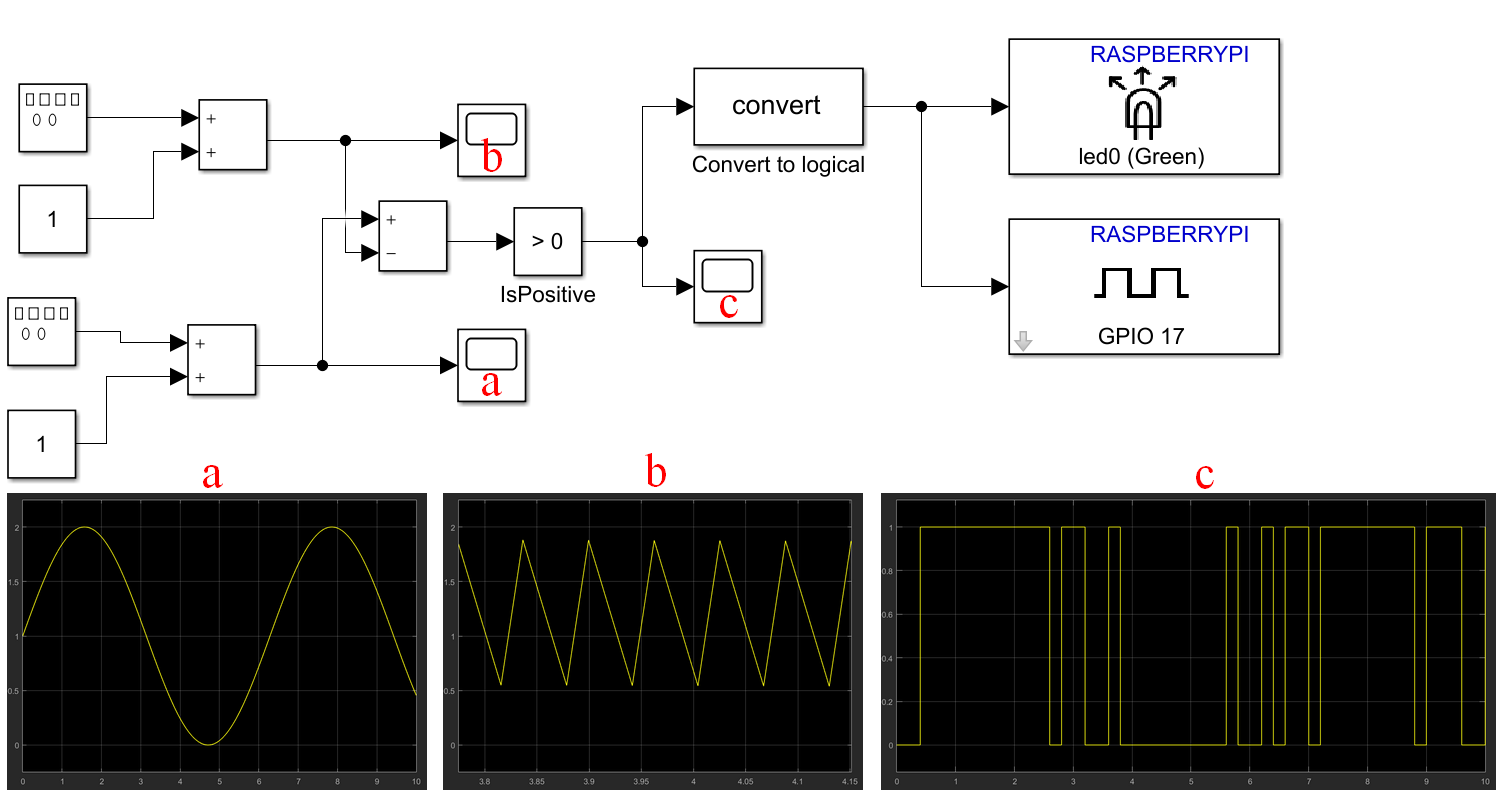
\includegraphics[scale=1]{img/saw.png}
  \caption{Sinusförmig verändernde Helligkeit}
  \label{fig:Sägezahnmodell zum Kreisförmigen Dimmungsverlauf einer LED}
\end{figure}
Dem Modell dienen zwei Impulsgebern als Input. Der untere in der Form einer Sinuskurve und der obere als Sägezähne. Anhand der Sägezähne lässt sich das Signal gut regulieren. Die Höhe der oberen Spitzen des Sägezahns ist dabei der maximale Impuls, der (in diesem Fall an LED und GPIO17) weitergegeben werden kann. Ziel dieses Beispieles ist es, anhand der Sinuskurve, das Signal jeweils so zu regulieren, dass das LED am hellsten ist, wenn die Sinuskurve einen Hochpunkt hat, das LED aus ist, bei einem niedrigen Maximalpunkt und dass das LED dazwischen jeweils so gedimmt ist, wie die aktuelle Position auf der Sinuskurve im Verhältnis zur Amplitude steht. Auf diese Weise lassen sich analoge Geräte wie Motoren von digitalen Schaltungen (die der Raspberry Pi wie alle anderen Microcontroller auch ausgibt) ansteuern. Abbildung 5.3 dient als Erklärungshilfe:
\begin{figure}[htb]
  \centering  
  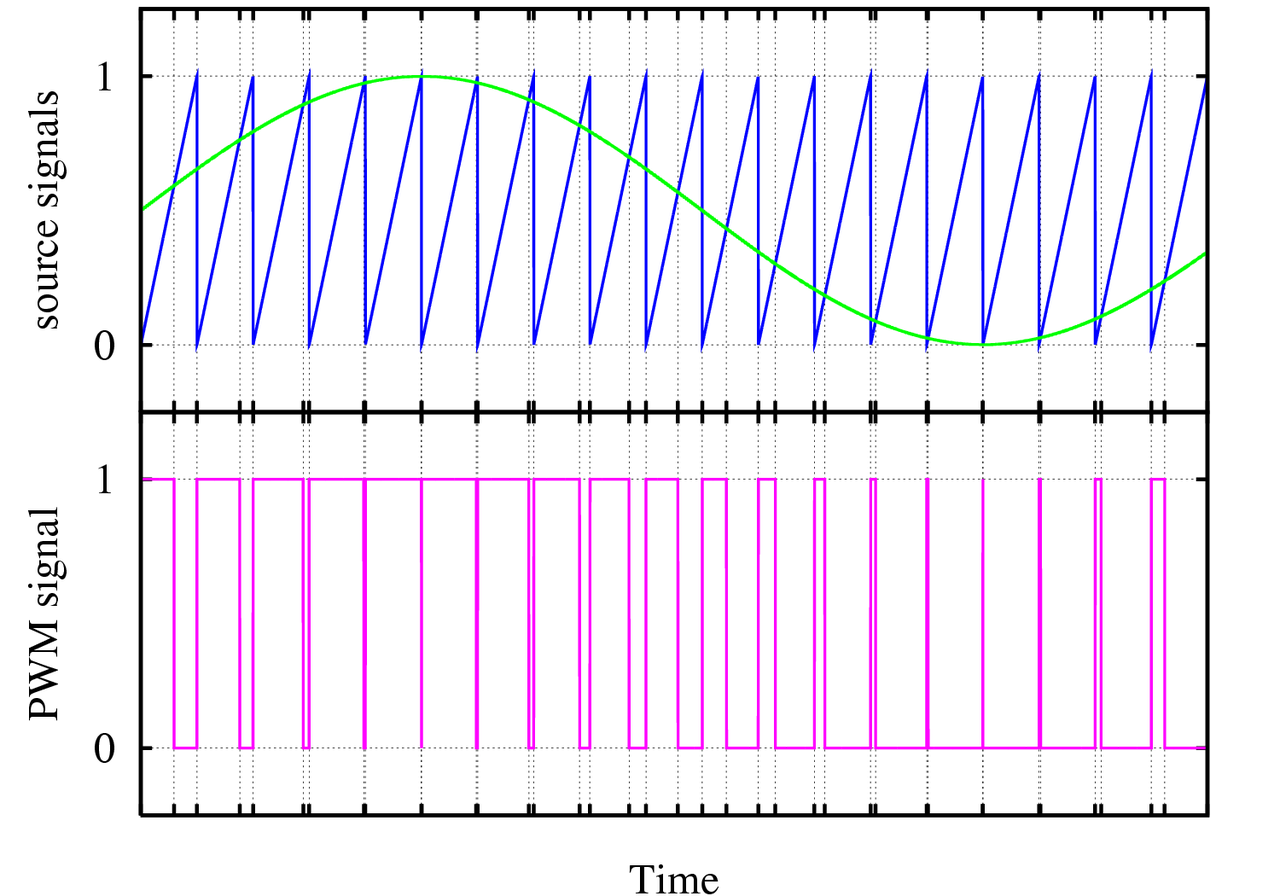
\includegraphics[scale=0.3]{img/sinussaw.png}
  \caption{Bei der Überlagerung von Sinuskurve und Sägezahnförmigem Signal, kann erstere durch die Schnittpunkte in ein analoges PWM-Signal umwandeln \\ Quelle: Wikipedia, \url{https://de.wikipedia.org/wiki/Pulsweitenmodulation}, stand 12.6.2018}
  \label{fig:Pulsweitenmodulation}
\end{figure}
Bei der Ausführung dieses Modells, ändert sich die Helligkeit der LED sinusartig. Das bedeutet dass die Pulsweitenmodulation funktioniert. Genau wie beim Test der LEDs, kann dieses Prinzip auch für einen Motor in Einsatz kommen, um dessen Drehmoment zu regulieren. So lässt sich jetzt nicht nur eine Sinuskurve umsetzten, sondern eben auch die gewünschten Geschwindigkeitsänderungen unseres Simulink-Modells. Statt der Sinuskurve als Eingang braucht man für die Realisierung der Geschwindigkeitsregelung am Raspberry Pi nur die aktuell gewünschte Soll-Geschwindigkeit anzugeben. Dies allerdings als Wert zwischen 0 und 1.  \\ \\

In diesem Kapitel wurde die Verbindung zwischen Modell und Hardware des Raspberry Pi erstellt und getestet. Genauer, es wurden die GPIOs des Raspberry Pi angesteuert, und überlegt, wie sich damit Motoren regeln lassen. Das zufriedenstellende Ergebnis war, dass sich mittels PWM die Aktuatoren (über die GPIOs) so regeln lassen, wie es für das Fahren eines Autos notwendig ist.




\chapter{Zusammenfassung und Ausblick}

\section{Fazit}
\label{sec:Fazit}
Das Ziel, ein System für das autonome Fahren zu modellieren, simulieren und entwerfen, wurde in dieser Arbeit vorgestellt. Ergebnis der Modellierung ist eine Reihe von Funktionen, die das Verhalten des Fahrzeugs versuchen möglichst genau und realistisch zu beschreiben. Die Simulation ergab, dass das Modell samt Reglung unter vorgegebener Koordinaten solide Ergebnisse liefert. Die Hardware Realisierung eines Prototypen erzielte ebenfalls zufriedenstellende Ergebnisse. \\


\section{Ausblick}
\label{sec:ausblick}
Ausgehend von dieser Arbeit könnte man weiter an dem System arbeiten und die Sensorik dafür integrieren. So ließe sich dann auch die Trajektorie vom System selbst bestimmen. Beides sind Vorschlage für Themen, bei denen meine Arbeit als Orientierung dienen kann. \\
Des Weiteren ließe sich unter Rücksichtnahme dieser Arbeit, leicht ein kompletter Prototyp fertigstellen, der vorgegebene Koordinaten abfährt. \\
Eine weitere Möglichkeit der Weiterführung dieser Arbeit wäre die Verwendung weiterer Modelle, als das hier vorgestellte Differentialantriebsmodell.

% pagestyle für gesamtes Dokument aktivieren
\pagestyle{fancy}


\begin{thebibliography}{9}
\bibitem[1] "Andreas Himmel, Viktoria Wiedmeyer, Juan Pablo Zometa, Michael Maiworm, 'oTToCAR', Otto-von-Guericke-Universität Magdeburg, Fakultät für Elektro- und Informationstechnik, Institut für Automatisierungstechnik, 29. November 2013

\bibitem[2] "Christian Rathgeber, 'Trajektorienplanung und -folgeregelung für assistiertes bis hochautomatisiertes Fahren', Hvon der Fakultät V – Verkehrs- und Maschinensysteme der Technischen Universität Berlin, 2016

\bibitem[3] "Dirk Reichardt, 'Kontinuierliche Verhaltenssteuerung eines autonomen Fahrzeugs in dynamischer Umgebung', Fachbereich Informatik der Universität Kaiserslautern, Januar 1996

\bibitem[4] "Dieter Schramm, Manfred Hiller, Roberto Bardini 'Modellbildung und Simulation der Dynamik von Kraftfahrzeugen', von der Universität Duisburg-Essen, ISBN 978-3-540-89313-4, 2010

\bibitem[5] "Fabian Freihube, 'Entwurf und Realisierung autonomer Fahrfunktionen in Modellfahrzeugen', HTWK Leipzig, Informatik, Mathematik und Naturwissenschaften, Oktober 2016

\bibitem[6] "Hans Pacejka, 'Tire and Vehicle Dynamics', Chapter 2 'Vehicle Dynamics Modeling', ISBN 9780080970165, 9. April 2012

\bibitem[7] "Magnus Rau, 'Koordination aktiver Fahrwerk-Regelsysteme zur Beeinflussung der Querdynamik mittels Verspannungslenkung', von der Fakultät Luft- und Raumfahrttechnik und Geodäsie der Universität Stuttgart, 01.06.2007

\bibitem[8]{ml}"MathWorks Stundent Competition Team, 'Differential Drive', \url{https://www.mathworks.com/examples/simmechanics/community/31986-differential-drive}, 2018

\bibitem[9] "Michael Graf, 'METHODE ZUR ERSTELLUNG UND ABSICHERUNG EINER MODELLBASIERTEN SOLLVORGABE FÜR FAHRDYNAMIKREGELSYSTEME', TECHNISCHE UNIVERSITÄT MÜNCHEN Fakultät für Maschinenwesen, Lehrstuhl für Fahrzeugtechnik, 27.06.2014

\bibitem[10]{robot} O. Bittel, 'Kinematik mobiler Roboter', HTWG Konstanz, WS 17/18

\bibitem[11] "Radionova L.V., Chernyshev A.D., 'Mathematical model of the vehicle in MATLAB Simulink', South Ural State University, 2015

\bibitem[12]{bild1}Statistisches Bundesamt Deutschland: "'Verkehrsunfälle - Fachserie 8 Reihe 7 - 2016"': Getötete nach Ortslagen 1973 - 2016

\bibitem[13]{link}Statistisches Bundesamt Deutschland: "'Fehlverhalten der Fahrzeugführer 2016"', \url{https://www.destatis.de/DE/ZahlenFakten/Wirtschaftsbereiche/TransportVerkehr/Verkehrsunfaelle/Verkehrsunfaelle.html}, 02.03.2018
   
\bibitem[14] "T. Bächle, K. Graichen,M. Buchholz, K. Dietmayer, 'Slip-Constrained Model Predictive Control Allocation for an All-Wheel Driven Electric Vehicle
', Institute of Measurement, Control and Microtechnology, University of Ulm, August 24-29, 2014

\end{thebibliography} 




\end{document}
